\chapter{Experimentos y resultados}\label{chapter5}

% **************************** Define Graphics Path **************************
\graphicspath{{Chapter5/Figs/}}


En este capítulo se describe la experimentación y lo resultados obtenidos
que muestran la mejora en el desempeño de un agente que aprende
con y sin información adicional de un grafo causal.
Para probar el concepto propuesto se atacan dos problemas: la tarea de clásica del taxi \cite{Dietterich:2000:HRL:1622262.1622268} y la de los
interruptores de luz, descrita en el capítulo \ref{chapter4}.
En resumen, los experimentos consisten en integrar el grafo $\mathcal{D}$ a la política $\epsilon$ greedy
en el algoritmo $Q$-learning \cite{watkins1992q}.
En la política $\epsilon$-greedy en vez de mantener fijo a $\epsilon$, se propone empezar motivando al agente a explorar y usar
el modelo causal e ir disminuyendo $\epsilon$ para dar más peso a la explotación.
Se comparan cuatro algoritmos, \textit{Q-learning sin información
adicional}, \textit{Q-learning con una estructural causal completa}, \textit{Q-learning con una estructura parcial} y un \textit{Q-learning con una estructura incorrecta}.
Dependiendo de la configuración experimental, cada uno de los algoritmos se ejecuta en una versión determinista y otra estocástica del ambiente. 
En las siguientes secciones se describen a detalle los experimentos realizados y los resultados. Todo el software desarrollado está 
disponible en \url{https://github.com/ivanfeliciano/causal_rl/}.


\section{Problema del taxi}

En esta sección se muestran los experimentos y resultados del método propuesto para el problema clásico del taxi \cite{Dietterich:2000:HRL:1622262.1622268}.
Se realiza un par de experimentos sobre dos configuraciones del ambiente diferentes,
una determinista y otra estocástica. De acuerdo con los resultados, 
el algoritmo usando un grafo causal como ``oráculo'' para seleccionar sus acciones
tiene un mejor desempeño en el ambiente determinista pero no hay una diferencia estadísticamente significativa en el ambiente estocástico.

\subsection{Descripción de la tarea}

El primer problema a resolver es la tarea clásica del taxi \cite{Dietterich:2000:HRL:1622262.1622268}.
La Figura \ref{fig:taxi} muestra gráficamente el problema.
Existen cuatro posiciones en el mundo marcadas como R, B, G, y Y. 
La tarea es episódica y en cada episodio, 
el taxi comienza en un cuadro aleatoriamente elegido. 
Existe un pasajero en una de la cuatro posiciones (también elegida
aleatoriamente), y el pasajero desea ser transportado a una de las
cuatro zonas.
El taxi debe dirigirse a la posición del pasajero, recogerlo, ir a su destino y dejarlo.
El episodio termina cuando el pasajero es dejado en su destino.

\begin{figure}[H]
    \centering
    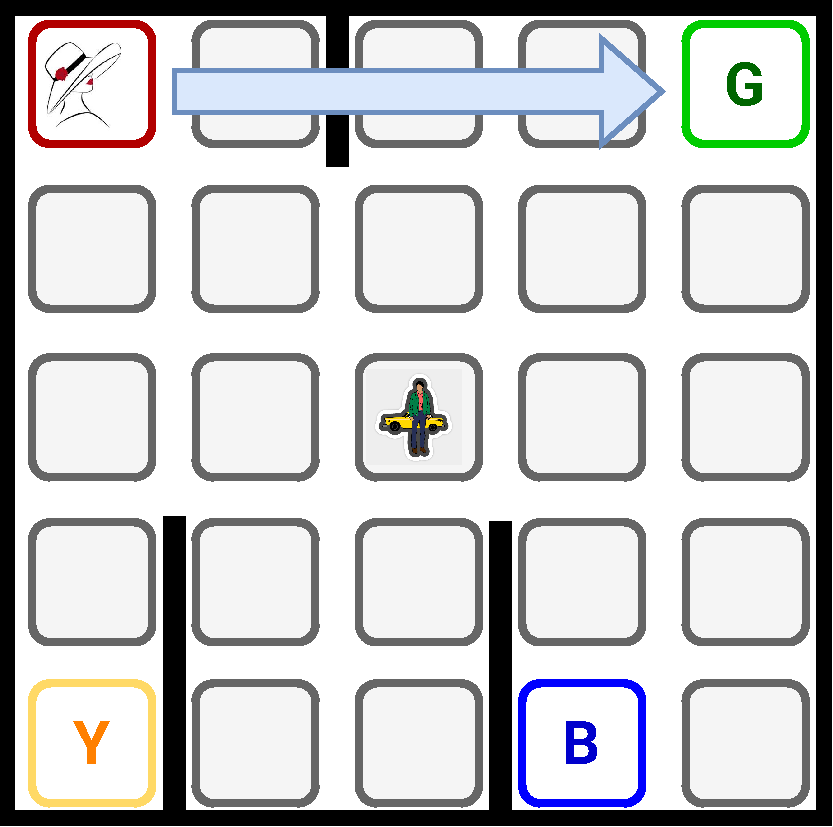
\includegraphics[scale=0.25]{Chapter5/Figs/taxi-env.pdf}
    \caption{La cuadrícula del ambiente del taxi. El taxi se encuentra en el cuadro central. En esta configuración del mundo, el objetivo es recoger al pasajero en la posición R y llevarlo a la posición G.}
    \label{fig:taxi}
\end{figure}

El conjunto de acciones $\mathcal{A}$ está compuesto por seis elementos: una acción para recoger $a_1$, una para dejar $a_2$ y
cuatro acciones de 
navegación que trasladan al taxi un cuadro al norte, sur, 
este u oeste, denotadas por $a_3, \dots, a_6$, respectivamente.
Existe una recompensa de -1 por cada acción, una recompensa adicional de 20 por cada pasajero llevado a su destino 
exitosamente y una penalización de -10 por acciones ilegales
de recolección y dejado.
El espacio de estados $\mathcal{S}$ tiene como elementos 
500 tuplas de tres elementos donde describen los 25 cuadros, las 5 posiciones del pasajero (incluyendo cuando está en el taxi) y los 4 destinos.


% Aquí ahondar más sobre el conjunto X y G, quienes lo compoenen y como está de pequeñito el problema
El conjunto $\mathcal{X}$ contiene 4 variables que traducen las tuplas con las posiciones del taxi y del pasajero en variables binarias. $x_1$
es la variable que dice si el taxi está en la misma posición que el
pasajero, $x_2$ es la variable que denota si el pasajero es llevado dentro del taxi, $x_3$ describe si el taxi está en la posición destino,
y $x_4$ es la variable que representa al estado de que el pasajero es entregado correctamente. Es una tarea relativamente simple y $x_1 \neq x_3$, por lo tanto las metas son $\mathcal{G} = \{\mathbf{g_1}, \mathbf{g_2}\}$, donde $\mathbf{g_1} = [1, 1, 0 , 0]$ y $\mathbf{g_2} = [0,1,1,1]$. El primer vector se puede ver como el sub objetivo de que el pasajero aborda el taxi y el segundo vector es la meta general, 
entregar al pasajero en su destino.
El grafo causal $\mathcal{D}$ entre las variables de acción y los estados se puede 
ver en la Figura \ref{fig:cm-taxi}. Para este problema, los efectos
necesitan de todas sus causas para suceder, por ejemplo, para que el
pasajero esté dentro del taxi, $x_2 = 1$, entonces se debe actuar
subiéndolo al vehículo $a_1$ y además estar en la misma ubicación que
el pasajero.

\begin{figure}[H]
    \centering
    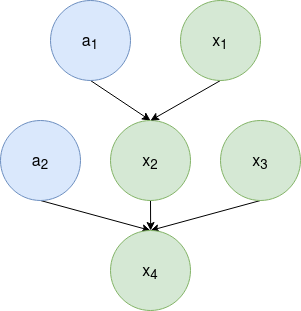
\includegraphics[scale=0.35]{Chapter5/Figs/causal_structure_taxi.png}
    \caption{Propuesta de una estructura causal para la tarea del taxi.}
    \label{fig:cm-taxi}
\end{figure}


\subsection{Configuración experimental}

Debido a la poca información que ofrece el grafo $\mathcal{D}$ y al tamaño de $\mathcal{G}$, para este problema no se ahonda en realizar experimentos con diferentes configuraciones. Por lo
tanto, sólo se comparan dos algoritmos,
el algoritmo Q-learning con y sin la estructura causal.
Además, los dos algoritmos se prueban sobre dos versiones del ambiente, una determinista
y otra estocástica. Los valores de los parámetros para los experimentos se muestran en el Cuadro \ref{tab:tax-params}. Se ejecutan $M$ experimentos y cada experimento consiste de ejecutar cada algoritmo $k$ de episodios. La medida
de desempeño es la recompensa promedio por episodio. El valor de $\epsilon$ se va decrementando en cada paso de tiempo de entrenamiento $t$ de forma lineal ($\epsilon = \max(\epsilon_{\min}, mt + \epsilon_{\max})$, $m < 0$ y representa la tasa de decremento)
con respecto al
número de episodios, por lo que se fomenta la exploración y el uso del modelo causal al principio y posteriormente se explota la información de $Q$.

\begin{table}[H]
\centering
\caption{Parámetros para las versiones del algoritmo Q-learning.}
\label{tab:tax-params}
\begin{tabular}{ll}
\hline
Parámetro                                                                                      & Valor    \\ \hline
$\alpha$                                                                                       & 0.8      \\
$\gamma$                                                                                       & 0.95     \\
$\epsilon_{\min}$                                                                              & 0.1      \\
$\epsilon_{\max}$                                                                              & 1.0      \\
$m$                                                                                            & -0.3e-04 \\
$k$                                                                                            & 1000     \\
$M$                                                                                            & 25       \\
\begin{tabular}[c]{@{}l@{}}Probabilidad de\\ transición en ambiente\\ estocástico\end{tabular} & 0.7      \\ \hline
\end{tabular}
\end{table}

\subsection{Resultados}

En la Figura \ref{fig:results-taxi} se muestran los resultados obtenidos
para ambas configuraciones del ambiente (determinista y estocástico) donde
los valores de los parámetros se describen en el Cuadro \ref{tab:tax-params}.
La recompensa promedio por episodio para el método propuesto y para el algoritmo
original Q-learning están en color naranja y azul, respectivamente. 
Los resultados muestran que el algoritmo Q-learning guiado por el grafo da un salto inicial alto y mantiene una recompensa promedio mucho mayor hasta que ambos métodos convergen. Esto es esperado, ya que
no inicia una exploración a ciegas. En ambas versiones del ambiente, los algoritmos parecen comportarse de manera similar a partir del episodio 400.

\begin{figure}[H]
  \centering
  \subfloat[Ambiente determinista.]{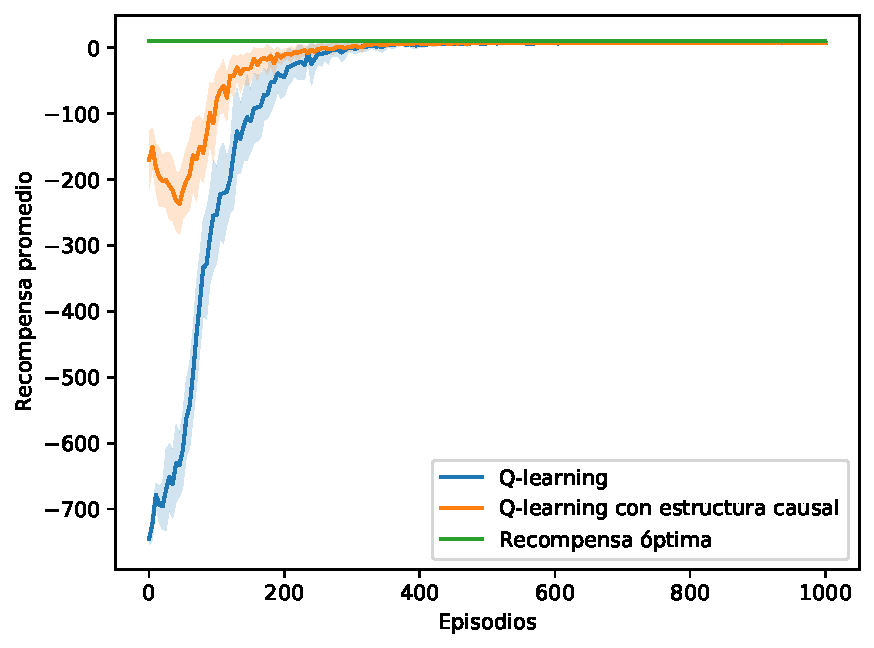
\includegraphics[width=0.45\textwidth]{Chapter5/Figs/taxi_env_comparison_det_1000_25_eps_30000.pdf}\label{fig:taxi-rew-det}}
  \hfill
  \subfloat[Ambiente estocástico.]{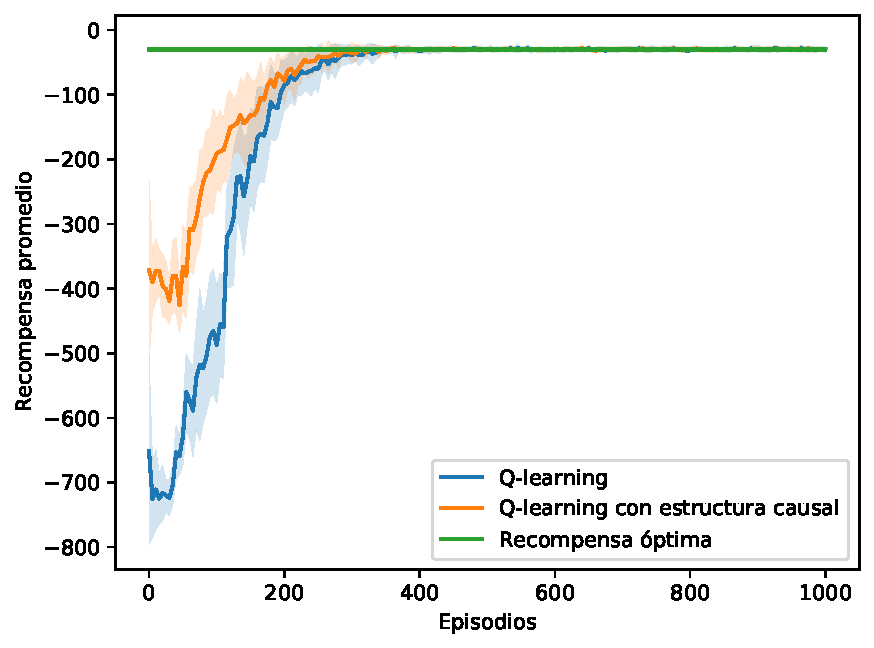
\includegraphics[width=0.45\textwidth]{Chapter5/Figs/taxi_env_comparison_sto_1000_25_eps_30000.pdf}\label{fig:taxi-rew-sto}}
  \caption{Comparación del desempeño para los dos algoritmos en 1000 episodios. La región sombreada es la desviación estándar para 50 experimentos.}
  \label{fig:results-taxi}
\end{figure}

La tarea para el ambiente determinista se considera resuelta cuando se obtiene una recompensa promedio de 9.7 durante 100 episodios consecutivos. Sin embargo, para fines de este experimentos se propone relajar este parámetro a un valor de 0 para el caso determinista y -30 para la versión estocástica del ambiente. En el Cuadro \ref{tab:resultados-taxi} se muestran los resultados del número de episodios, promedio sobre $M$ experimentos,
que tarda cada algoritmo en alcanzar la recompensa óptima propuesta durante una racha de más de 100 episodios. Entre menor sea el número de episodios en alcanzar la racha denota que un algoritmo aprendió más rápido.

De acuerdo con los resultados del Cuadro \ref{tab:resultados-taxi}, el algoritmo que alcanza la recompensa óptima antes, es el método Q-learning con la información causal. Sin embargo, con el fin de validar los resultados se utiliza la prueba de Welch como se sugiere en \cite{colas2019hitchhikers}. La hipótesis nula $h_0$ corresponde a que el número de episodios en alcanzar la recompensa óptima durante más de 100 episodios seguidos es igual para ambos algoritmos. Para el caso del ambiente determinista la hipótesis es rechazada con $p < 0.05$. Sin embargo, para el caso del ambiente estocástico se falla al rechazar $h_0$ ya que $p > 0.05$. Por lo tanto, a pesar de que los resultados en el Cuando 
\ref{tab:resultados-taxi} indican un mejor comportamiento para el algoritmo con la estructura causal auxiliando la selección de acciones, no hay diferencia estadísticamente significativa en la versión estocástica del ambiente.

% Please add the following required packages to your document preamble:
% \usepackage{booktabs}
\begin{table}[!h]
\centering
\caption{Resultados del número de episodios promedio y la desviación estándar en alcanzar una recompensa > 0 con una racha > 100 y > -30 con una racha > 100 para los ambientes determinista y estocástico, respectivamente.}
\label{tab:resultados-taxi}
\begin{tabular}{@{}lll@{}}
\toprule
Algoritmo & \begin{tabular}[c]{@{}l@{}}Ambiente determinista.\\ Número de episodios\end{tabular} & \begin{tabular}[c]{@{}l@{}}Ambiente estocástico.\\ Número de episodios\end{tabular} \\ \midrule
Q-learning & $632 \pm 69$ & $496 \pm 247$ \\
\begin{tabular}[c]{@{}l@{}}Q-learning +\\ estructura causal\end{tabular} & $\mathbf{589 \pm 106}$ & $476 \pm 232$ \\ \bottomrule
\end{tabular}
\end{table}

Los resultados obtenidos son intuitivos, esto es, comenzar una exploración a ciegas es 
peor que conocer un poco del mundo por eso el valor de recompensa inicial mayor del algoritmo propuesto. 
% Por otro lado, ambos algoritmos se comportan de manera similar después de unos cientos de episodios.
Por otro lado, la información del mundo con el que cuenta el agente es muy limitada. En realidad solo se cuenta con la información de lo que provocan dos de las seis acciones posibles. Esto puede ser la razón por la que la diferencia entre los algoritmos 
en un ambiente estocástico no es significativa. Tener un modelo pequeño sumando un ambiente donde no siempre intentar una acción te lleva a un estado deseado conduce a un paso de exploración más. Esto por lo tanto, provoca que ambos algoritmos sean muy parecidos.
 
\section{Problema de los interruptores de luz}

En esta sección se muestran los experimentos y resultados del método propuesto para
el problema de los interruptores de luz descrito en el capítulo \ref{chapter4}.
A diferencia del ambiente del taxi, este problema cuenta 
con diferentes variaciones. Por ejemplo,
diferentes tipos de conexiones en la estructura subyacente del problema, el tamaño de dicha estructura, etc.
En general, de acuerdo con los experimentos, el algoritmo usando un grafo causal como ``oráculo'' para seleccionar sus acciones tiene un mejor desempeño incluso en 
configuraciones donde las estructuras causales están parcialmente incorrectas o también 
al disminuir la tasa de consultas al modelo en una parte temprana del aprendizaje.


\subsection{Descripción de la tarea}
Para los experimentos de esta sección se ataca la tarea de control de interruptores de luz propuesta en \cite{nair2019causal} y descrita de manera general en la Sección \ref{section:switches-example}. Un agente tiene el control
de $N$ interruptores que controlan $N$ luces en un sitio.
Cada acción $a\in \mathcal{A}$ corresponde a mover un interruptor o 
a no mover ninguno, por lo tanto $|\mathcal{A}| = N + 1$.
El agente puede percibir dos tipos de señales del ambiente,
una imagen $s$ con una vista cenital del sitio, o vectores binarios $x \in \{0,1\}^N$ de 
macro-variables que codifican las luces prendidas, donde
$x_i = 1$ si la luz en la zona $i$ está prendida, de otro modo 
toma el valor $x_i = 0$.

Se exploran tres tipos de estructuras causales entre los
interruptores y las luces: \textit{uno-a-uno},
\textit{causa común} y \textit{efecto común}.
En los problemas con estructuras uno-a-uno cada interruptor corresponde a una sola luz.
Para el segundo tipo, de causa común, todas
las luces son controladas a lo más por un interruptor pero un
solo interruptor puede controlar más de una luz.
El tercer caso son estructuras de efecto común, donde cada interruptor
controla una sola luz, aunque múltiples interruptores
pueden controlar la misma luz. De manera visual, los tres tipos de estructuras
se muestran en la Figura \ref{fig:struct}.

\begin{figure}[H]
    \centering
    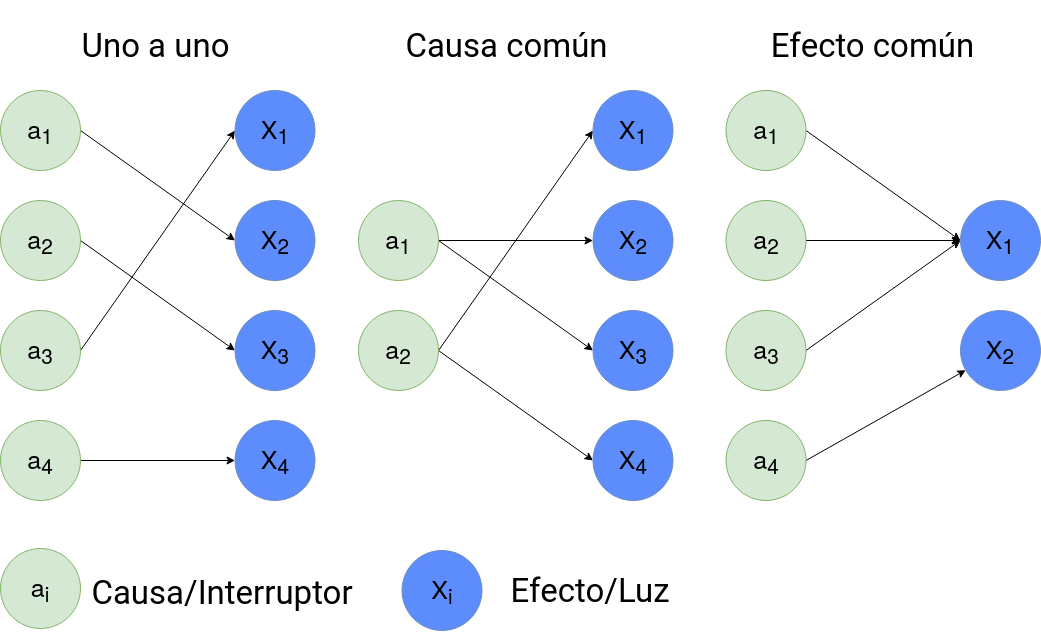
\includegraphics[scale=0.3]{Chapter5/Figs/switches_struct.png}
    \caption{Tipos de estructuras causales subyacentes posibles.}
    \label{fig:struct}
\end{figure}
La recompensa inmediata $r$ brindada al agente se calcula obteniendo la distancia entre el vector de variables de estado alto nivel $\mathbf{x}$ y el vector meta $\mathbf{g}$. En este problema se usa la distancia euclidiana.


\subsection{Configuración experimental general}

En las siguientes secciones se compara el desempeño 
del método propuesto en diferentes escenarios, principalmente, para mostrar 
las posibilidades y ventajas de usar un información del grafo causal, completa, incompleta e incluso incorrecta. 
% A pesar de ser diferentes
% experimentos, éstos comparten la configuración de algunos elementos, por ejemplo, 
% la medida de desempeño, el número de variables $N$, etc.
Se comparan cuatro algoritmos, teniendo como base
el método Q-learning. Donde la diferencia subyace en la cantidad y calidad de la información adicional con la que cuenta. A continuación, se describen de manera breve los métodos
comparados.

\begin{itemize}
    \item \textit{Q-learning sin información adicional} ($Q_1$). Este método sirve como
    línea de base para medir que tanto mejora el aprendizaje. El algoritmo, dependiendo del espacio de estados sobre el que se trabaje, es el 
    método básico de Q-learning \cite{watkins1992q} o Q-learning profundo \cite{mnih2013playing}, para estados
    discretos y continuos, respectivamente. La selección de acciones se lleva a cabo mediante una política $\epsilon$ greedy clásica.
    \item \textit{Q-learning + estructura causal completa}($Q_2$). Durante la política de selección de acciones, el agente cuenta con la estructura causal del ambiente completa y verdadera $\mathcal{D}$.
    \item \textit{Q-learning + estructura causal incompleta}($Q_3$). En este caso, el agente cuenta con un subgrafo $\mathcal{D'}$ del grafo $\mathcal{D}$. Este subgrafo se genera eliminando aristas de $\mathcal{D}$ aleatoriamente.
    \item \textit{Q-learning + estructura causal incorrecta}($Q_4$). Este algoritmo consulta un modelo $\mathcal{D}''$ con relaciones espurias y sin algunas relaciones verdaderas. Este grafo $\mathcal{D}''$ se obtiene generando un subgrafo de $\mathcal{D}$ como en el caso anterior y agregando aristas aleatoriamente.
\end{itemize}

\begin{figure}
  \centering
  \subfloat[$\mathcal{D}$.]{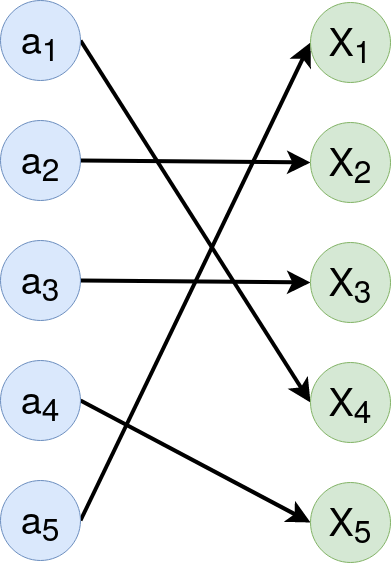
\includegraphics[width=0.2\textwidth]{Chapter5/Figs/completeD.png}\label{fig:completeD}}
  \qquad
  \subfloat[$\mathcal{D}'$]{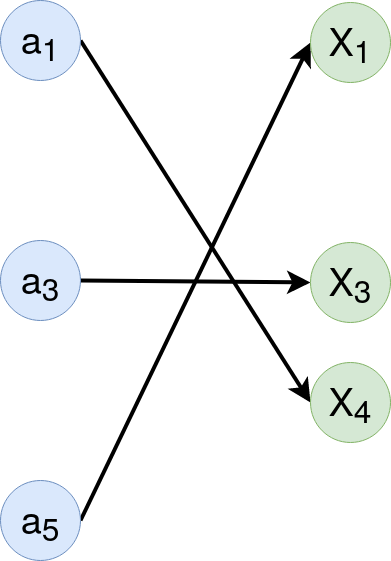
\includegraphics[width=0.2\textwidth]{Chapter5/Figs/incompleteD.png}\label{fig:incompleteD}}
%   \hfill
    \qquad
  \subfloat[$\mathcal{D}''$]{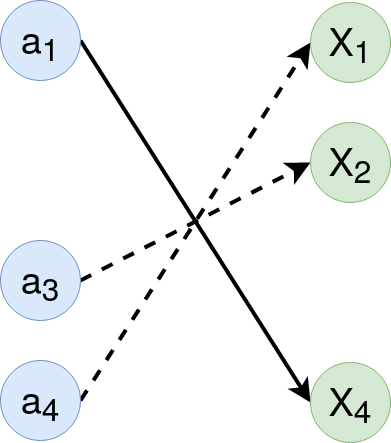
\includegraphics[width=0.2\textwidth]{Chapter5/Figs/wrongD.png}\label{fig:wrongD}}
  \caption{Ejemplo de los tres tipos de información con los que puede  contar el algoritmo Q-learning. El tipo de estructura
  del problema es uno-a-uno. Las aristas dirigidas punteadas describen conexiones espurias.}
  \label{fig:types-info-dag}
\end{figure}

Para medir el desempeño de los algoritmos se evalúa la recompensa
promedio sobre una serie de experimentos.
Cada experimento consiste en ejecutar el algoritmo de aprendizaje durante $k$ episodios, en 
un ambiente con una estructura causal fija $\mathcal{D}$ y donde se busca alcanzar la meta $\mathbf{g}$.
La recompensa promedio para el $i$ ésimo episodio está dada por
$R^{i} = \frac{1}{H}\sum_{t=0}^H r(\mathbf{x}_t, \mathbf{g})$,
donde $H$ corresponde al tamaño del episodio.
El vector $\mathbf{R_i}$, del $i$ ésimo experimento contiene las recompensas promedio por cada episodio, y se define como
$\mathbf{R_i} = (R^{1}, \dots, R^k)$.

Finalmente, la medida de comparación entre algoritmos es
el promedio de los vectores $\mathbf{R_i}$, $i\in [1, M]$,  obtenidos en $M$ experimentos. Esta medida, denotada como  $average$ puede escribirse como 
\begin{equation}
\label{eq:average}
average(\mathbf{R_1}, \dots, \mathbf{R_M}) = \frac{1}{M}(\sum^M_i \mathbf{R_{i}^1}, \dots, \sum^M_i\mathbf{R_{i}^k}),    
\end{equation}

donde $M$ es el número de experimentos y el $\mathbf{R_i^j}$ indica la recompensa promedio obtenida en el $j$ ésimo episodio del $i$ ésimo experimento.

El parámetro $\epsilon$ se disminuye linealmente, donde
en cada selección de acción va decreciendo hasta llegar
un valor mínimo. La regla de actualización de $\epsilon$ en
el paso de tiempo $t$ se puede definir como $\epsilon = \max(\epsilon_{\min}, (\epsilon_{\min} - \epsilon_{\max}) \times t/ (N \times k \times \delta) + \epsilon_{\max})$. Donde $0 < \delta \leq 1$, es un factor para controlar
que tan rápido se alcanza el valor de $\epsilon$  mínimo, entre más cercano a 0,
termina más rápido la exploración.
% Con excepción
% del Experimento 2 (Sección \ref{subsection:exp-epsilon}), donde se cambia el denominador de la
% tasa de decremento para que éste se más rápido.

%Los experimentos se llevan a cabo en dos versiones del ambiente, una discreta y otra estocástica. 
De manera general se realizan tres tipos de experimentos. El primer experimento tiene 
como objetivo medir el desempeño al modificar la estructura causal $\mathcal{D}$ a diferentes porcentajes para obtener $\mathcal{D'}$ y $\mathcal{D}''$. El segundo experimento es con respecto a cambiar la tasa de decremento
de $\epsilon$ para llegar más rápido o lento a explotar 
más constantemente. El tercer experimento, es probar
el algoritmo cuando no se tienen las variables
de alto nivel como observaciones directas, por lo tanto,
se trabaja sobre un espacio de estados continuo. En general,
algunos de los parámetros que se comparten entre los experimentos se muestran en el Cuadro \ref{tab:switch-params}.

\begin{table}[H]
\centering
\caption{Valores para algunos parámetros de los algoritmos.}
\label{tab:switch-params}
\begin{tabular}{ll}
\hline
Parámetro                                                                                      & Valor    \\ \hline
$\alpha$                                                                                       & 0.8      \\
$\gamma$                                                                                       & 0.95     \\
$\epsilon_{\min}$                                                                              & 0.1      \\
$\epsilon_{\max}$                                                                              & 1.0      \\
$N$                                                                                            & \{5, 7, 9\} \\
$H$                                                                                            & \{5, 7, 9\} \\
$k$                                                                                            & \{200, 5000, 10000, 20000\}\\
$M$                                                                                            & 10       \\
\begin{tabular}[c]{@{}l@{}}Probabilidad de\\ transición en ambientes\\ estocástico\end{tabular} & 0.75      \\ \hline
\end{tabular}
\end{table}

\clearpage
\subsection{Variando el porcentaje de modificación del grafo causal}\label{exp1}

Se realiza una serie de experimentos donde se busca mostrar el comportamiento 
del método propuesto sobre subgrafos del grafo causal verdadero. Estos subgrafos son generados a partir del $\mathcal{D}$, alterándolo a diferentes niveles.

\subsubsection{Configuración experimental}

\begin{itemize}
    \item El espacio de estados es discreto, es decir, el agente puede
    obtener las variables $\mathcal{X}$ directamente del ambiente.
    \item Se prueba modificando el grafo $\mathcal{D}$ para obtener a los
    grafos $\mathcal{D'}$ y $\mathcal{D''}$ en tres niveles. El porcentaje de nivel de cambio se representa con el parámetro $p_{mod}$.
    Para cada nivel, el subgrafo $\mathcal{D'}$ se genera al remover un porcentaje $p_{mod}$ de las aristas en el grafo $\mathcal{D}$. Para producir $\mathcal{D''}$ se elimina $p_{mod}$ de las aristas y después, de la mitad de conexiones perdidas, se crean nuevas diferentes a las iniciales.
    \begin{itemize}
        \item Nivel bajo de modificación, $p_{mod} = 25 \%$.
        \item Nivel medio de modificación. $p_{mod} = 50 \%$.
        \item Nivel alto de modificación. $p_{mod} = 75 \%$
    \end{itemize}
    \item Se examina sobre los tres tipos de estructuras posibles: uno-a-uno, 
    causa común y efecto común. 
    \item Se prueba sobre ambientes deterministas y estocásticos.
    
    \item La tasa de exploración está dada por un $\delta = 0.5$ lo que indica que aproximadamente a mitad del entrenamiento la probabilidad de explotación alcanza su máximo valor.
\end{itemize}

\subsubsection{Objetivo}

Determinar si la información provista por un modelo
incompleto o parcialmente incorrecto ayuda y no
afecta negativamente el desempeño del algoritmo de RL.

\subsubsection{Hipótesis}

Dado que la información del modelo causal solo guía la selección
de acciones durante la exploración, entonces un grafo con escasos
datos correctos sigue siendo mejor que una búsqueda aleatoria. 
% En el
% peor caso, el algoritmo se comportaría como el método sin información adicional.


\subsubsection{Resultados}

Para comparar el desempeño de los distintos algoritmos propuestos
para todas las diferentes configuraciones del experimento
se evalúa la medida \textit{average} descrita anteriormente.
De manera gráfica se puede ver el desempeño de los algoritmos
para los diferentes valores de $p_{mod}$ y tipo de ambiente en las Figuras \ref{fig:low-mod-det}, \ref{fig:low-mod-sto}, \ref{fig:med-mod-det}, \ref{fig:med-mod-sto},  \ref{fig:high-mod-det} y \ref{fig:high-mod-sto}.

De acuerdo con las Figuras \ref{fig:low-mod-det}-\ref{fig:high-mod-sto}
en la mayoría de los casos los algoritmos que utilizan conocimiento del grafo inician con una recompensa mayor y se estabilizan más rápido que el algoritmo Q-learning
sin información adicional en ambientes con transiciones deterministas y estocásticas. Para el caso donde $p_{mod} = 25$, los algoritmos con información incompleta e incorrecta parecen 
comportarse de manera muy similar. Esto puede ser debido 
a que la tasa de alteración del grafo es muy baja y  a que $N$ no toma
valores muy grandes, por lo que hay muy poca diferencia entre el grafo incompleto y el incorrecto. 
En el caso de $p_{mod} = 50$, se
puede notar que el desempeño de los algoritmos
con información incompleta e incorrecta se 
va moviendo en dirección a la curva del algoritmo
Q-learning sin información extra.
Finalmente, para $p_{mod} = 75$,  a pesar de haber modificado el grafo 
causal en un porcentaje bastante alto, la poca información que queda y es correcta sigue siendo suficiente para alcanzar una recompensa mayor mucho más rápido, donde al menos es más notable para las estructuras de tipo causa común y de efecto común.
Existe un comportamiento extraño en las tareas con una estructura del tipo uno a uno. Se puede ver que entre más crece el valor de $N$ los algoritmos que utilizan el grafo tienden a decrecer en dirección al punto de transición en el que la explotación llega a su máximo valor. Sin embargo, una vez que pasa ese punto, los algoritmos se siguen comportando de manera superior al algoritmo clásico.


Por otro lado, además de la colección de medidas en forma de curvas de aprendizaje, se propone hacer una comparación estadística de
los métodos. Para llevar a cabo esta última, se compara la recompensa promedio de los últimos $E$ episodios
de entrenamiento sobre los $M$ experimentos. Con esto, se 
puede obtener una muestra de tamaño $E$ para cada algoritmo
y hacer una prueba estadística para mostrar que existe una diferencia entre ellos. Principalmente, es de interés saber si los algoritmos que utilizan información extra son superiores 
al algoritmo Q-learning usando una exploración a prueba y error. 

En las tablas \ref{tab:pmo-one-to-one}, \ref{tab:pmo-one-to-many} y \ref{tab:pmo-many-to-one} se muestran
los promedios de las recompensas durante los últimos $E$ episodios. En casi todos las tareas el algoritmo Q-learning usando el grafo causal completo tiene una recompensa mayor que en los otros métodos. En general, todos los métodos que utilizan el grafo ya sea incorrecto o incompleto superan al método clásico de Q-learning. Se utiliza la prueba de Welch con $p < 0.05$ para encontrar diferencias estadísticamente significativas como se sugiere en \cite{colas2019hitchhikers}. Las pruebas solo se realizan comparando los resultados del algoritmo simple Q-learning con cada uno de los otros métodos. Los resultados de las pruebas indican que sí existe una diferencia estadística en el desempeño de los algoritmos, excluyendo algunos casos donde se obtiene un valor $p\geq 0.05$ (marcados por $\dagger$ en las tablas). Dichos casos aparecen en los experimentos donde las alteración del grafo $\mathcal{D}$ es un porcentaje $p_{mod} = 75$ y además se agregan relaciones espurias. Esto es de esperarse ya que entre más se modifica el grafo correcto se aproxima la búsqueda de acciones a una exploración aleatoria.
\newpage

\begin{table}[h]
\centering
\caption{Comparación de la recompensa promedio obtenida durante los últimos $E=100$ episodios de entrenamiento para $M$ experimentos en tareas con estructuras causales uno a uno.}
\label{tab:pmo-one-to-one}
\resizebox{\textwidth}{!}{%
\begin{tabular}{@{}ccclll@{}}
\toprule
Ambiente & $p_{mod}$ & Algoritmo & \multicolumn{3}{c}{$N$} \\ \cmidrule(l){4-6} 
 &  &  & \multicolumn{1}{c}{5} & \multicolumn{1}{c}{7} & \multicolumn{1}{c}{9} \\ \midrule
Determinista & $25\%$ & $Q_{1}$ & $-2.2182 \pm 0.6336$ & $-4.2527 \pm 0.9449$ & $-6.4783 \pm 1.0360$ \\
 &  & $Q_{2}$ & $\mathbf{-1.8956 \pm 0.5285}$ & $\mathbf{-3.4366 \pm 0.7290}$ & $-5.5112 \pm 1.0322$ \\
 &  & $Q_{3}$ & $-1.9240 \pm 0.4748$ & $-3.5972 \pm 0.7493$ & $\mathbf{-5.2752 \pm 0.8429}$ \\
 &  & $Q_{4}$ & $-1.9818 \pm 0.4810$ & $-3.5400 \pm 0.6413$ & $-5.6452 \pm 0.8337$ \\ \cmidrule(l){2-6} 
 & $50\%$ & $Q_{1}$ & $-2.2628 \pm 0.5568$ & $-4.3893 \pm 0.9663$ & $-6.4983 \pm 1.1034$ \\
 &  & $Q_{2}$ & $\mathbf{-1.9269 \pm 0.5063}$ & $\mathbf{-3.3805 \pm 0.6799}$ & $\mathbf{-5.3568 \pm 1.0327}$ \\
 &  & $Q_{3}$ & $-2.0227 \pm 0.5103$ & $-3.6810 \pm 0.7031$ & $-5.5596 \pm 0.9284$ \\
 &  & $Q_{4}$ & $-2.0515 \pm 0.5205$ & $-3.7771 \pm 0.8140$ & $-5.7934 \pm 1.0148$ \\ \cmidrule(l){2-6} 
 & $75\%$ & $Q_{1}$ & $-2.3585 \pm 0.6444$ & $-4.3475 \pm 0.8879$ & $-6.4210 \pm 1.1059$ \\
 &  & $Q_{2}$ & $\mathbf{-1.8609 \pm 0.4570}$ & $\mathbf{-3.4178 \pm 0.7382}$ & $\mathbf{-5.4319 \pm 0.9450}$ \\
 &  & $Q_{3}$ & $-2.1248 \pm 0.5040$ & $-3.8530 \pm 0.8418$ & $-5.8715 \pm 1.0626$ \\
 &  & $Q_{4}$ & $-2.1903 \pm 0.6093\dagger$ & $-4.0736 \pm 0.8175$ & $-6.2007 \pm 0.9860\dagger$ \\ \midrule
Estocástico & $25\%$ & $Q_{1}$ & $-5.1114 \pm 0.9096$ & $-9.1281 \pm 1.1897$ & $-14.1541 \pm 1.5689$ \\
 &  & $Q_{2}$ & $\mathbf{-3.7371 \pm 0.8183}$ & $\mathbf{-6.9731 \pm 1.2073}$ & $\mathbf{-9.6946 \pm 1.7353}$ \\
 &  & $Q_{3}$ & $-3.8397 \pm 0.9062$ & $-7.4121 \pm 1.1744$ & $-11.2450 \pm 1.7928$ \\
 &  & $Q_{4}$ & $-3.7755 \pm 0.7262$ & $-7.4194 \pm 1.3376$ & $-11.3526 \pm 1.9065$ \\ \cmidrule(l){2-6} 
 & $50\%$ & $Q_{1}$ & $-4.8947 \pm 0.7977$ & $-9.2118 \pm 1.2497$ & $-13.8851 \pm 1.5869$ \\
 &  & $Q_{2}$ & $\mathbf{-3.5493 \pm 0.8052}$ & $\mathbf{-7.3603 \pm 1.3592}$ & $\mathbf{-10.1254 \pm 1.8590}$ \\
 &  & $Q_{3}$ & $-4.0995 \pm 0.8538$ & $-8.0543 \pm 1.2003$ & $-12.2734 \pm 1.5236$ \\
 &  & $Q_{4}$ & $-4.0742 \pm 1.0099$ & $-7.8257 \pm 1.2826$ & $-11.9317 \pm 1.6780$ \\ \cmidrule(l){2-6} 
 & $75\%$ & $Q_{1}$ & $-4.7275 \pm 0.8827$ & $-9.0077 \pm 1.1266$ & $-13.8726 \pm 1.5532$ \\
 &  & $Q_{2}$ & $\mathbf{-3.4796 \pm 0.7879}$ & $\mathbf{-6.9571 \pm 1.4064}$ & $\mathbf{-9.8165 \pm 1.9188}$ \\
 &  & $Q_{3}$ & $-4.2609 \pm 0.8242$ & $-8.5903 \pm 1.2043$ & $-12.5843 \pm 1.7400$ \\
 &  & $Q_{4}$ & $-4.2405 \pm 0.9147$ & $-8.7413 \pm 1.4550\dagger$ & $-12.9938 \pm 1.4176$ \\ \bottomrule
\end{tabular}%
}
\end{table}

\newpage
\begin{table}[h]
\centering
\caption{Comparación de la recompensa promedio obtenida durante los últimos $E=100$ episodios de entrenamiento para $M$ experimentos en tareas con estructuras causales del tipo causa común.}
\label{tab:pmo-many-to-one}
\resizebox{\textwidth}{!}{%
\begin{tabular}{@{}ccclll@{}}
\toprule
Ambiente & $p_{mod}$ & Algoritmo & \multicolumn{3}{c}{$N$} \\ \cmidrule(l){4-6} 
 &  &  & \multicolumn{1}{c}{5} & \multicolumn{1}{c}{7} & \multicolumn{1}{c}{9} \\ \midrule
Determinista & $25\%$ & $Q_{1}$ & $-1.1605 \pm 0.4370$ & $-2.3821 \pm 0.5554$ & $-3.6241 \pm 0.8354$ \\
 &  & $Q_{2}$ & $\mathbf{-0.8818 \pm 0.2987}$ & $\mathbf{-1.8817 \pm 0.5535}$ & $\mathbf{-2.9917 \pm 0.6222}$ \\
 &  & $Q_{3}$ & $-0.8999 \pm 0.3342$ & $-1.8906 \pm 0.5059$ & $-3.1555 \pm 0.7857$ \\
 &  & $Q_{4}$ & $-0.9052 \pm 0.3063$ & $-1.9772 \pm 0.5410$ & $-3.1813 \pm 0.6925$ \\ \cmidrule(l){2-6} 
 & $50\%$ & $Q_{1}$ & $-1.2611 \pm 0.4208$ & $-2.2211 \pm 0.6455$ & $-2.8791 \pm 0.7447$ \\
 &  & $Q_{2}$ & $\mathbf{-0.9493 \pm 0.2981}$ & $\mathbf{-1.6838 \pm 0.4796}$ & $\mathbf{-2.2900 \pm 0.5628}$ \\
 &  & $Q_{3}$ & $-1.0367 \pm 0.3289$ & $-1.8876 \pm 0.5945$ & $-2.4913 \pm 0.7249$ \\
 &  & $Q_{4}$ & $-1.0658 \pm 0.4114$ & $-1.8973 \pm 0.5475$ & $-2.8104 \pm 0.7954\dagger$ \\ \cmidrule(l){2-6} 
 & $75\%$ & $Q_{1}$ & $-1.3095 \pm 0.4857$ & $-2.4471 \pm 0.6858$ & $-3.7470 \pm 0.9684$ \\
 &  & $Q_{2}$ & $\mathbf{-1.0618 \pm 0.3104}$ & $\mathbf{-1.9527 \pm 0.5322}$ & $\mathbf{-3.0603 \pm 0.6601}$ \\
 &  & $Q_{3}$ & $-1.1391 \pm 0.3324$ & $-2.1410 \pm 0.5985$ & $-3.4041 \pm 0.8123$ \\
 &  & $Q_{4}$ & $-1.2016 \pm 0.4291\dagger$ & $-2.4146 \pm 0.6697\dagger$ & $-3.5423 \pm 0.7628\dagger$ \\ \midrule
Estocástico & $25\%$ & $Q_{1}$ & $-3.0886 \pm 0.9845$ & $-6.1796 \pm 1.6089$ & $-9.2795 \pm 2.0556$ \\
 &  & $Q_{2}$ & $\mathbf{-2.1093 \pm 0.6978}$ & $\mathbf{-4.2816 \pm 1.1846}$ & $\mathbf{-5.2987 \pm 1.4281}$ \\
 &  & $Q_{3}$ & $-2.2082 \pm 0.7754$ & $-4.4287 \pm 1.0685$ & $-5.6103 \pm 1.4823$ \\
 &  & $Q_{4}$ & $-2.2333 \pm 0.7078$ & $-4.4320 \pm 1.2439$ & $-5.4898 \pm 1.5539$ \\ \cmidrule(l){2-6} 
 & $50\%$ & $Q_{1}$ & $-2.9996 \pm 1.0511$ & $-6.0544 \pm 1.2444$ & $-8.4563 \pm 1.8175$ \\
 &  & $Q_{2}$ & $\mathbf{-2.1329 \pm 0.7398}$ & $\mathbf{-4.1256 \pm 1.2303}$ & $\mathbf{-5.8154 \pm 1.4156}$ \\
 &  & $Q_{3}$ & $-2.4228 \pm 0.7311$ & $-4.6498 \pm 1.1331$ & $-6.9922 \pm 1.6813$ \\
 &  & $Q_{4}$ & $-2.4134 \pm 0.8149$ & $-4.1292 \pm 1.1034$ & $-6.5562 \pm 1.4675$ \\ \cmidrule(l){2-6} 
 & $75\%$ & $Q_{1}$ & $-3.0753 \pm 0.8946$ & $-5.6907 \pm 1.3626$ & $-9.0473 \pm 2.0631$ \\
 &  & $Q_{2}$ & $\mathbf{-2.1460 \pm 0.7327}$ & $\mathbf{-3.6353 \pm 1.1232}$ & $\mathbf{-5.3417 \pm 1.3045}$ \\
 &  & $Q_{3}$ & $-2.2385 \pm 0.7288$ & $-4.8728 \pm 1.1800$ & $-6.3821 \pm 1.3441$ \\
 &  & $Q_{4}$ & $-2.3781 \pm 0.8174$ & $-4.3506 \pm 1.2888$ & $-6.8824 \pm 1.8552$ \\ \bottomrule
\end{tabular}%
}
\end{table}

\newpage
\begin{table}[h]
\centering
\caption{Comparación de la recompensa promedio obtenida durante los últimos $E=100$ episodios de entrenamiento para $M$ experimentos en tareas con estructuras causales de efecto común.}
\label{tab:pmo-one-to-many}
\resizebox{\textwidth}{!}{%
\begin{tabular}{@{}ccclll@{}}
\toprule
Ambiente & $p_{mod}$ & Algoritmo & \multicolumn{3}{c}{$N$} \\ \cmidrule(l){4-6} 
 &  &  & \multicolumn{1}{c}{5} & \multicolumn{1}{c}{7} & \multicolumn{1}{c}{9} \\ \midrule
Determinista & $25\%$ & $Q_{1}$ & $-1.1566 \pm 0.4032$ & $-2.0655 \pm 0.5925$ & $-2.5841 \pm 0.6171$ \\
 &  & $Q_{2}$ & $\mathbf{-0.9035 \pm 0.2978}$ & $\mathbf{-1.6037 \pm 0.4009}$ & $\mathbf{-2.1047 \pm 0.5454}$ \\
 &  & $Q_{3}$ & $-0.9295 \pm 0.3044$ & $-1.6527 \pm 0.5065$ & $-2.1139 \pm 0.5718$ \\
 &  & $Q_{4}$ & $-0.9903 \pm 0.3278$ & $-1.6576 \pm 0.4356$ & $-2.3156 \pm 0.5591$ \\ \cmidrule(l){2-6} 
 & $50\%$ & $Q_{1}$ & $-1.1123 \pm 0.4498$ & $-2.0584 \pm 0.6533$ & $-2.9029 \pm 0.7290$ \\
 &  & $Q_{2}$ & $\mathbf{-0.8622 \pm 0.2878}$ & $\mathbf{-1.6729 \pm 0.4784}$ & $\mathbf{-2.3992 \pm 0.5821}$ \\
 &  & $Q_{3}$ & $-0.9735 \pm 0.3656$ & $-1.8843 \pm 0.4881$ & $-2.5665 \pm 0.5631$ \\
 &  & $Q_{4}$ & $-1.0127 \pm 0.3423\dagger$ & $-2.0133 \pm 0.5224\dagger$ & $-2.6393 \pm 0.7003$ \\ \cmidrule(l){2-6} 
 & $75\%$ & $Q_{1}$ & $-0.9944 \pm 0.3483$ & $-2.3420 \pm 0.6175$ & $-3.2112 \pm 0.7041$ \\
 &  & $Q_{2}$ & $\mathbf{-0.7371 \pm 0.2555}$ & $\mathbf{-1.8766 \pm 0.4679}$ & $\mathbf{-2.5704 \pm 0.5597}$ \\
 &  & $Q_{3}$ & $-0.8670 \pm 0.3424$ & $-2.1462 \pm 0.5880$ & $-2.8315 \pm 0.6618$ \\
 &  & $Q_{4}$ & $-0.8988 \pm 0.3557\dagger$ & $-2.2513 \pm 0.5743\dagger$ & $-3.0330 \pm 0.6829\dagger$ \\ \midrule
Estocástico & $25\%$ & $Q_{1}$ & $-2.4246 \pm 0.7587$ & $-4.9754 \pm 1.2124$ & $-7.7349 \pm 1.4403$ \\
 &  & $Q_{2}$ & $\mathbf{-1.6373 \pm 0.6081}$ & $-3.5762 \pm 1.0292$ & $\mathbf{-4.8947 \pm 1.4667}$ \\
 &  & $Q_{3}$ & $-1.8670 \pm 0.6335$ & $-3.6253 \pm 1.0470$ & $-5.6975 \pm 1.3601$ \\
 &  & $Q_{4}$ & $-1.8538 \pm 0.5879$ & $\mathbf{-3.5423 \pm 0.9738}$ & $-4.9075 \pm 1.3517$ \\ \cmidrule(l){2-6} 
 & $50\%$ & $Q_{1}$ & $-2.3026 \pm 0.6698$ & $-5.0139 \pm 1.0946$ & $-7.8808 \pm 1.3351$ \\
 &  & $Q_{2}$ & $\mathbf{-1.4379 \pm 0.4905}$ & $-3.3055 \pm 0.9801$ & $\mathbf{-5.4403 \pm 1.3450}$ \\
 &  & $Q_{3}$ & $-1.6029 \pm 0.5111$ & $-3.4351 \pm 0.9925$ & $-5.9440 \pm 1.4399$ \\
 &  & $Q_{4}$ & $-1.7097 \pm 0.6777$ & $\mathbf{-3.2720 \pm 0.9536}$ & $-6.5544 \pm 1.4985$ \\ \cmidrule(l){2-6} 
 & $75\%$ & $Q_{1}$ & $-2.3648 \pm 0.7404$ & $-5.1371 \pm 1.1200$ & $-7.6762 \pm 1.5876$ \\
 &  & $Q_{2}$ & $\mathbf{-1.7755 \pm 0.5862}$ & $\mathbf{-3.2939 \pm 0.9156}$ & $\mathbf{-4.9183 \pm 1.2352}$ \\
 &  & $Q_{3}$ & $-2.2238 \pm 0.6873\dagger$ & $-4.2950 \pm 1.1680$ & $-6.2311 \pm 1.5134$ \\
 &  & $Q_{4}$ & $-2.1695 \pm 0.6820\dagger$ & $-4.1598 \pm 1.0756$ & $-6.1031 \pm 1.3614$ \\ \bottomrule
\end{tabular}%
}
\end{table}

%%%%%%%%%%%%%%%%%
%%%PMOD 25 DET%%%
%%%%%%%%%%%%%%%%%
\begin{figure}
\settoheight{\tempdima}{\includegraphics[width=.32\linewidth]{example-image-a}}%
\centering\begin{tabular}{@{}c@{ }c@{ }c@{ }c@{}}
&\textbf{Uno-a-uno} & \textbf{Causa común} & \textbf{Efecto común} \\
\rowname{$N = 5$}&
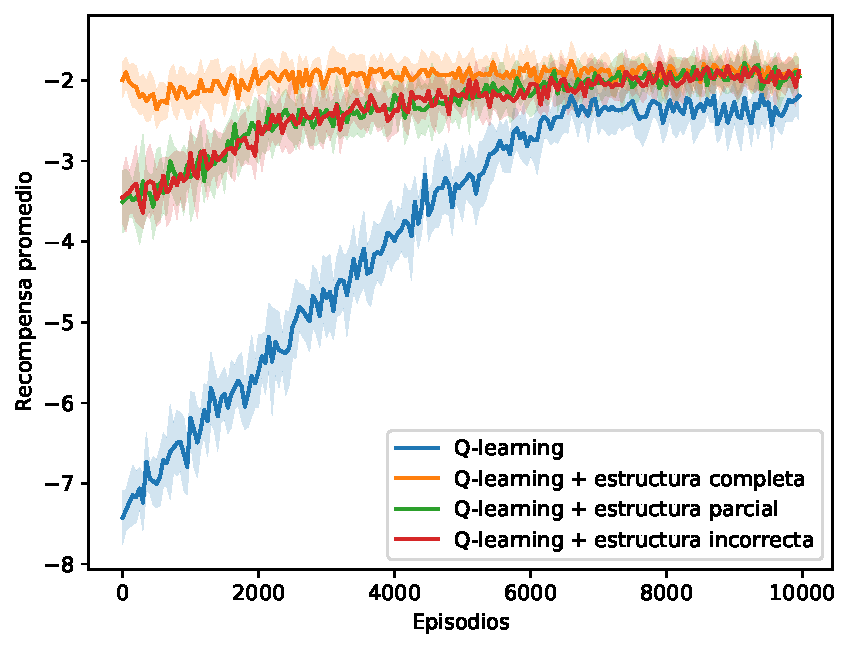
\includegraphics[width=.32\linewidth]{Chapter5/Figs/modexp/deterministic_low_025_one_to_one_N_5_experiments_10_episodes_10000_eps_25000.pdf}&
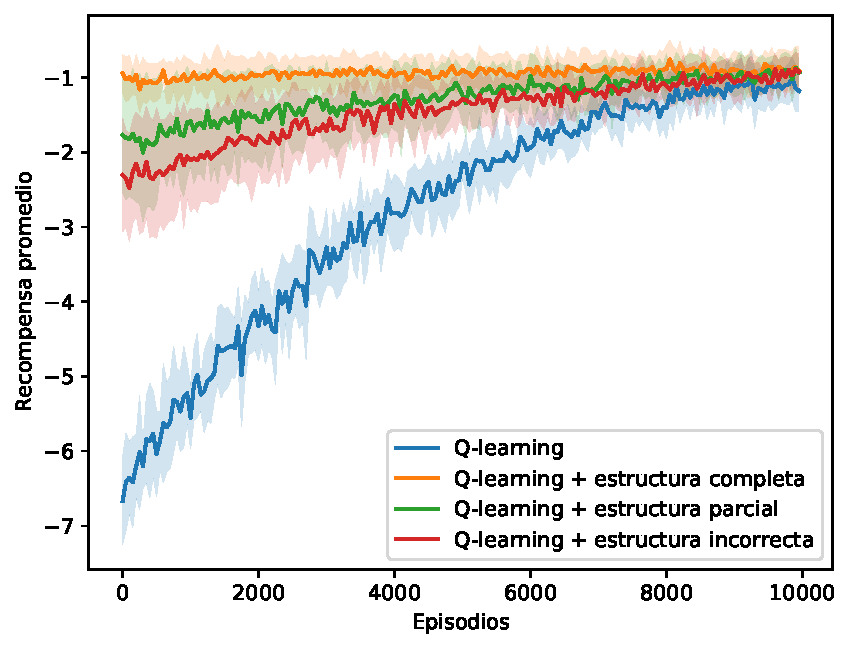
\includegraphics[width=.32\linewidth]{Chapter5/Figs/modexp/deterministic_low_025_one_to_many_N_5_experiments_10_episodes_10000_eps_25000.pdf}&
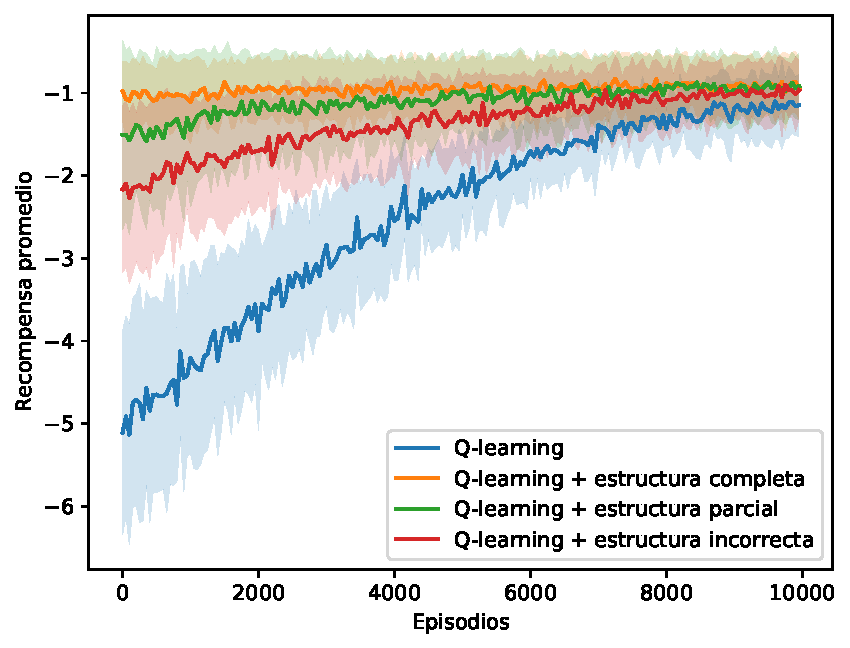
\includegraphics[width=.32\linewidth]{Chapter5/Figs/modexp/deterministic_low_025_many_to_one_N_5_experiments_10_episodes_10000_eps_25000.pdf}
\\
\rowname{$N=7$}&
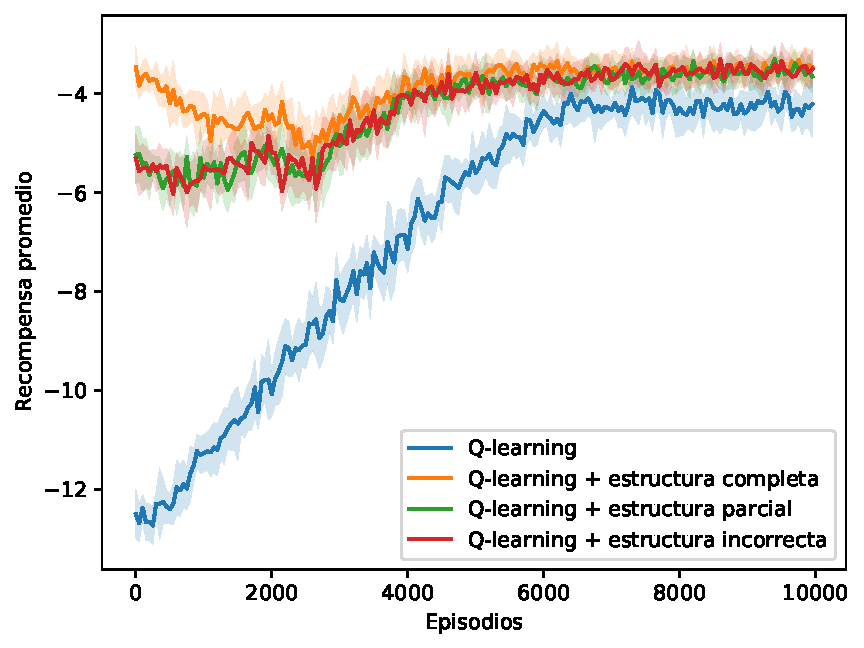
\includegraphics[width=.32\linewidth]{Chapter5/Figs/modexp/deterministic_low_025_one_to_one_N_7_experiments_10_episodes_10000_eps_35000.pdf}&
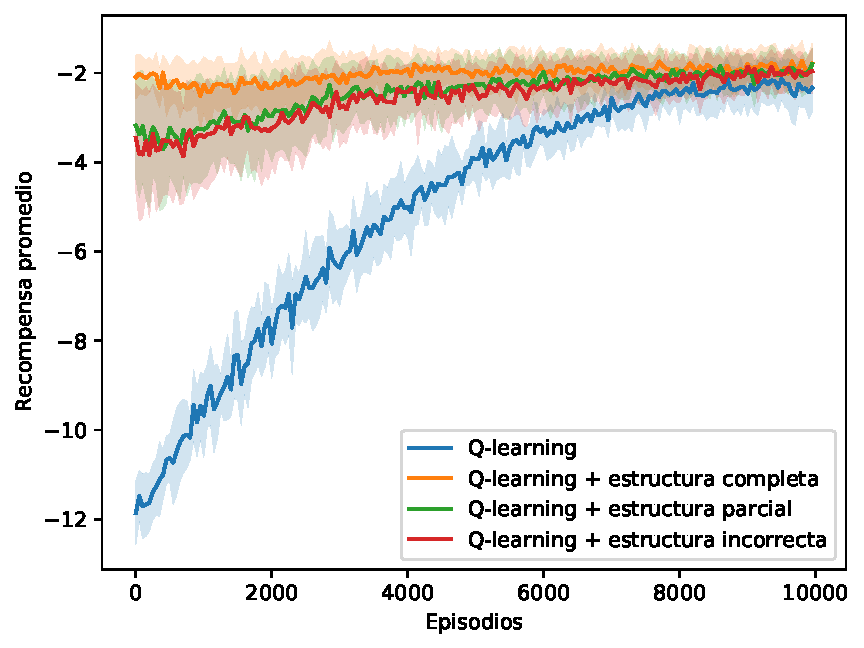
\includegraphics[width=.32\linewidth]{Chapter5/Figs/modexp/deterministic_low_025_one_to_many_N_7_experiments_10_episodes_10000_eps_35000.pdf}&
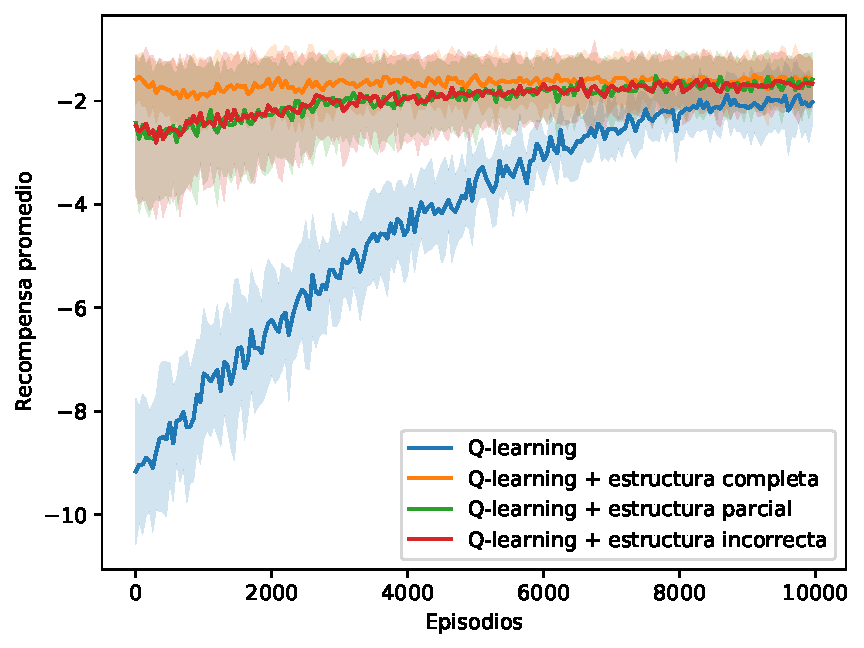
\includegraphics[width=.32\linewidth]{Chapter5/Figs/modexp/deterministic_low_025_many_to_one_N_7_experiments_10_episodes_10000_eps_35000.pdf}
\\
\rowname{$N = 9$}&

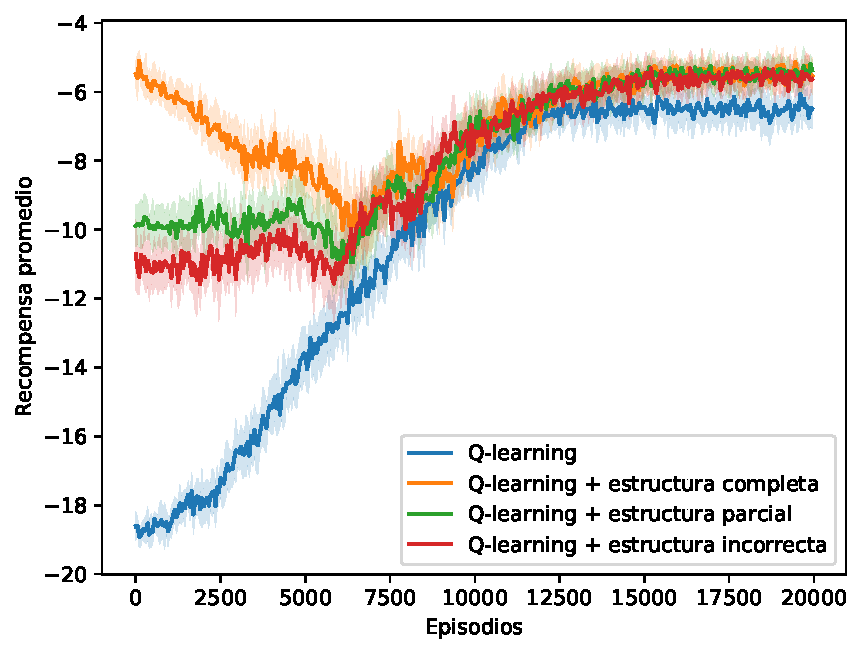
\includegraphics[width=.32\linewidth]{Chapter5/Figs/modexp/deterministic_low_025_one_to_one_N_9_experiments_10_episodes_20000_eps_90000.pdf}&
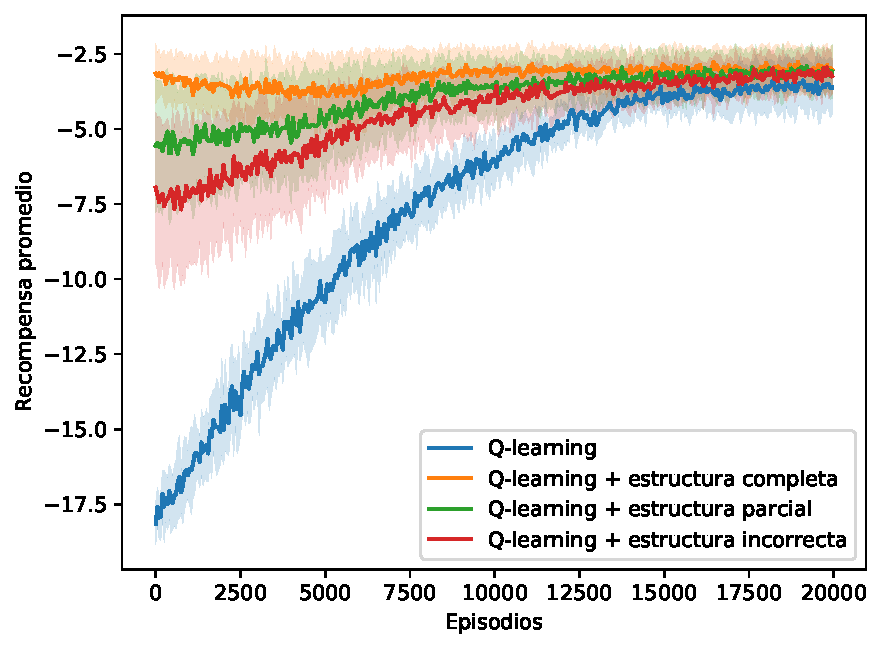
\includegraphics[width=.32\linewidth]{Chapter5/Figs/modexp/deterministic_low_025_one_to_many_N_9_experiments_10_episodes_20000_eps_90000.pdf}&
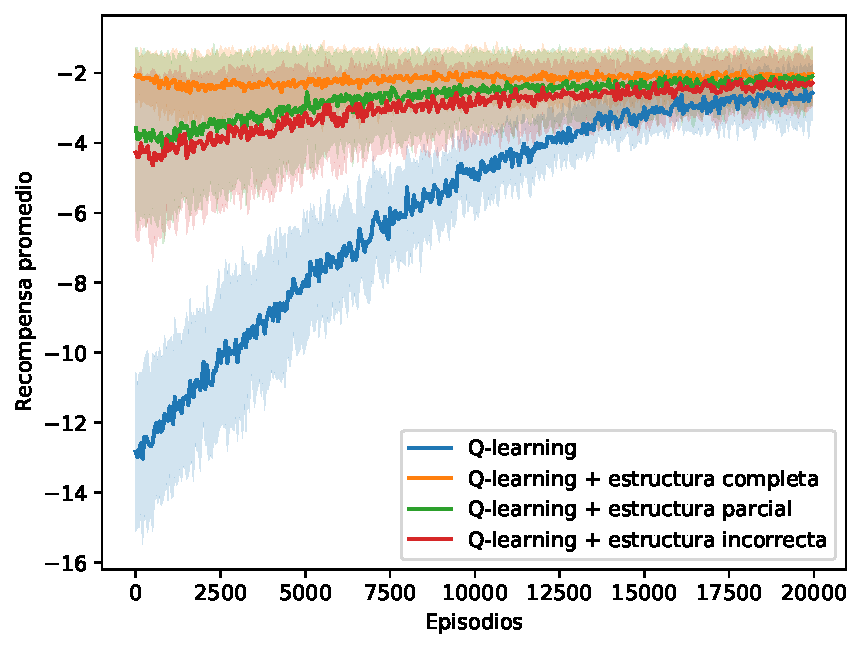
\includegraphics[width=.32\linewidth]{Chapter5/Figs/modexp/deterministic_low_025_many_to_one_N_9_experiments_10_episodes_20000_eps_90000.pdf}

\end{tabular}
\caption{Comparación del desempeño para los 4 algoritmos con un nivel de alteración $p_{mod} = 25 \%$ en un ambiente determinista. Las gráficas muestran la medida $average$ y la desviación estándar (región sombreada) para 10 experimentos con 10000 (para $N = 5, 7$) y 20000 (para $N = 9$) episodios.}
\label{fig:low-mod-det}
\end{figure}

%%%%%%%%%%%%%%%%%
%%%PMOD 25 STO%%%
%%%%%%%%%%%%%%%%%
\begin{figure}
\settoheight{\tempdima}{\includegraphics[width=.32\linewidth]{example-image-a}}%
\centering\begin{tabular}{@{}c@{ }c@{ }c@{ }c@{}}
&\textbf{Uno-a-uno} & \textbf{Causa común} & \textbf{Efecto común} \\
\rowname{$N = 5$}&
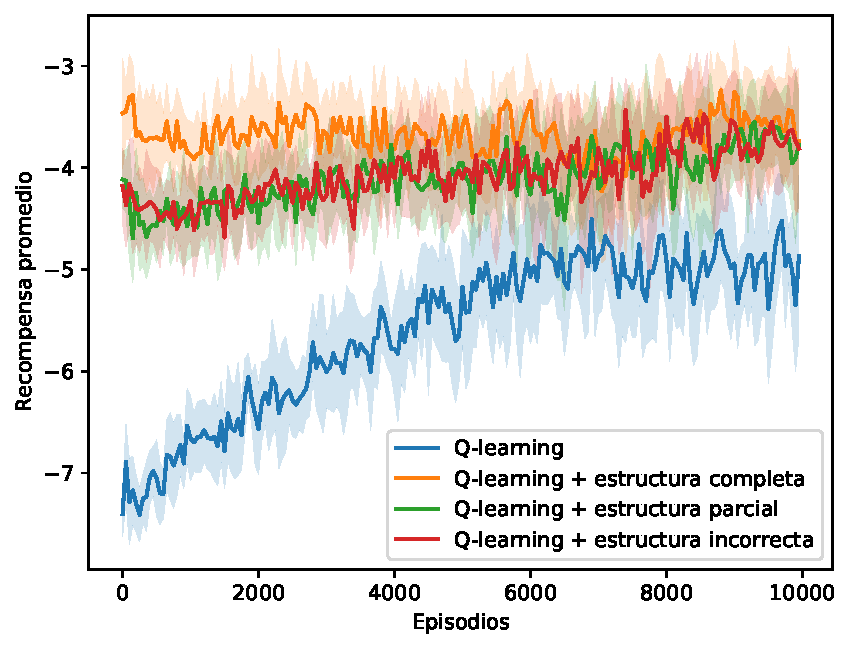
\includegraphics[width=.32\linewidth]{Chapter5/Figs/modexp/stochastic_low_025_one_to_one_N_5_experiments_10_episodes_10000_eps_25000.pdf}&
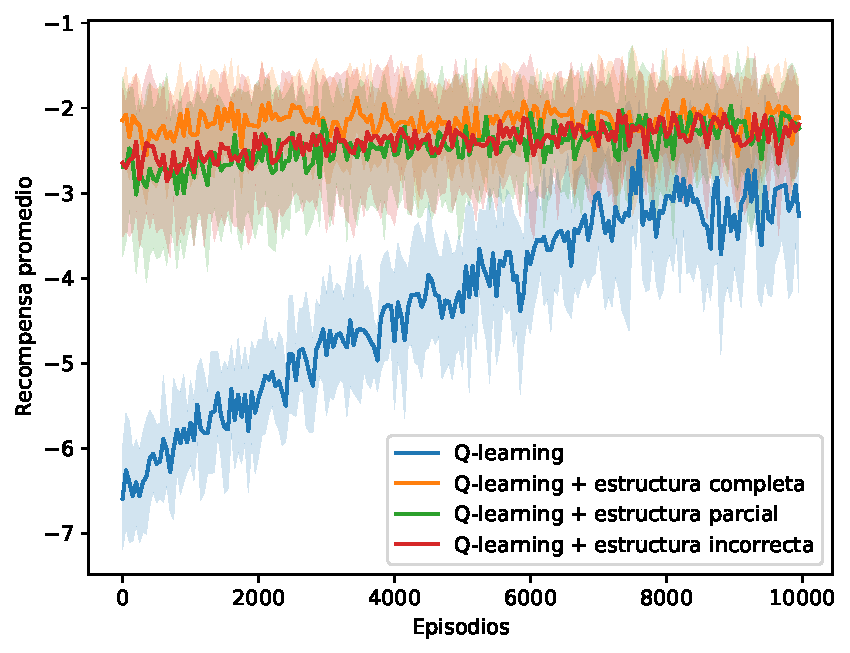
\includegraphics[width=.32\linewidth]{Chapter5/Figs/modexp/stochastic_low_025_one_to_many_N_5_experiments_10_episodes_10000_eps_25000.pdf}&
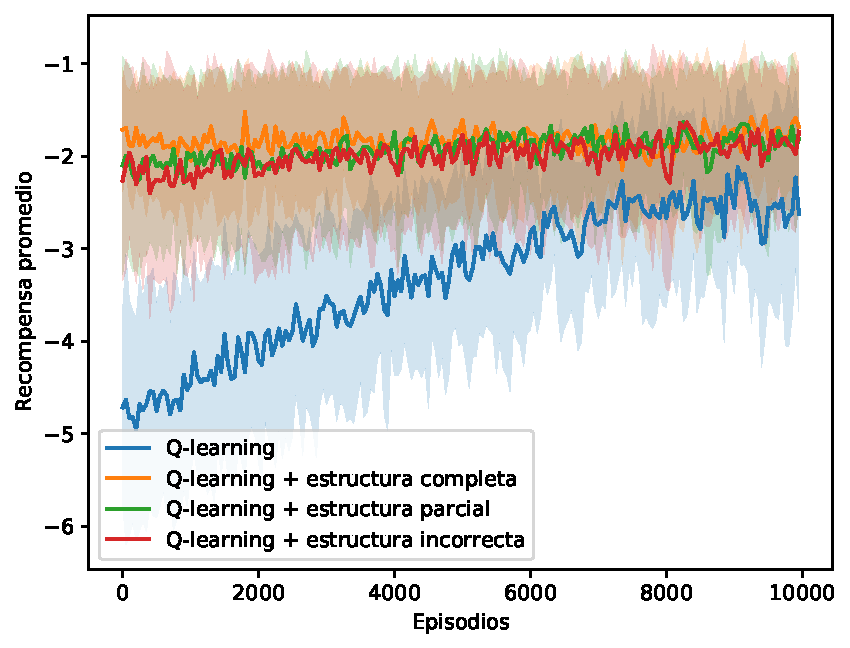
\includegraphics[width=.32\linewidth]{Chapter5/Figs/modexp/stochastic_low_025_many_to_one_N_5_experiments_10_episodes_10000_eps_25000.pdf}
\\
\rowname{$N=7$}&
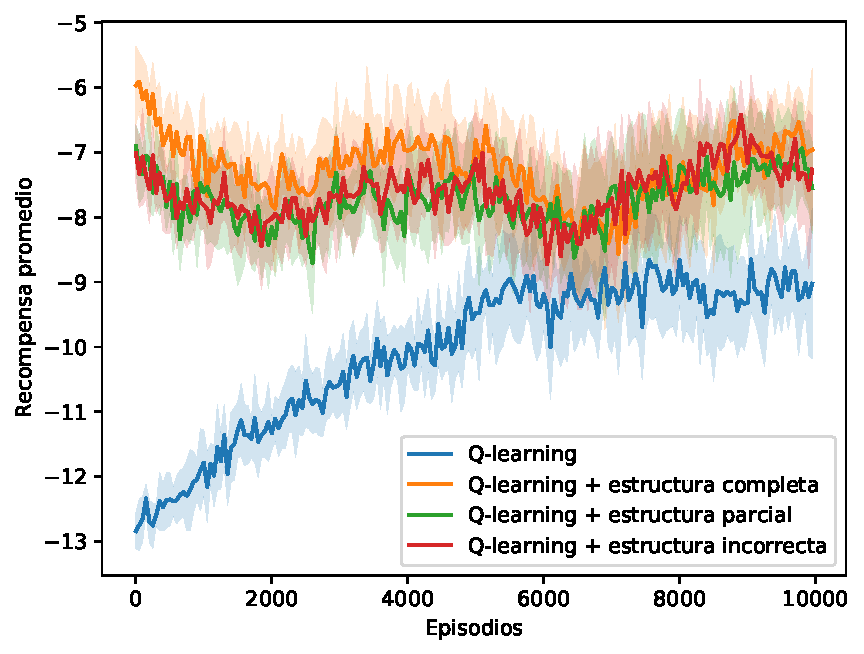
\includegraphics[width=.32\linewidth]{Chapter5/Figs/modexp/stochastic_low_025_one_to_one_N_7_experiments_10_episodes_10000_eps_35000.pdf}&
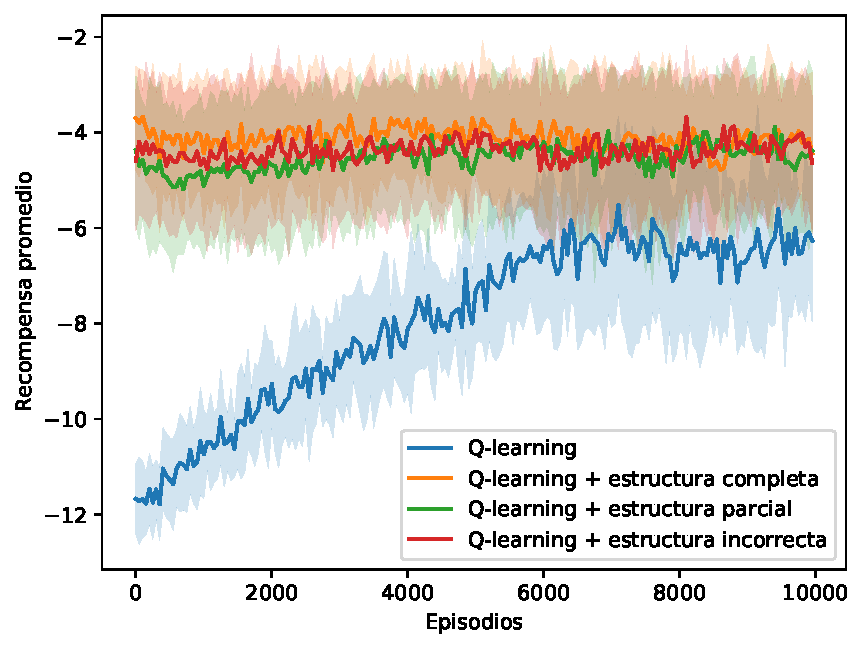
\includegraphics[width=.32\linewidth]{Chapter5/Figs/modexp/stochastic_low_025_one_to_many_N_7_experiments_10_episodes_10000_eps_35000.pdf}&
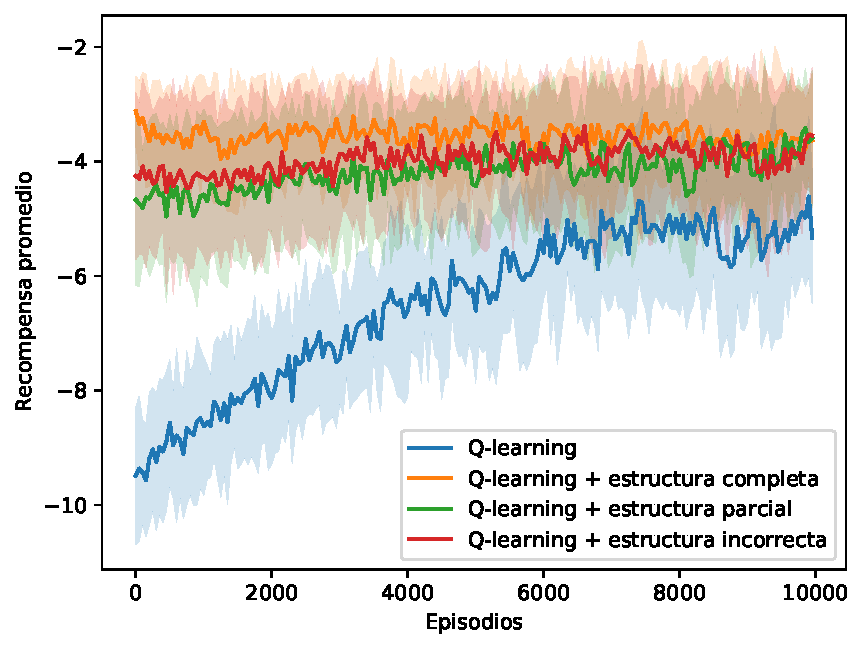
\includegraphics[width=.32\linewidth]{Chapter5/Figs/modexp/stochastic_low_025_many_to_one_N_7_experiments_10_episodes_10000_eps_35000.pdf}
\\
\rowname{$N = 9$}&

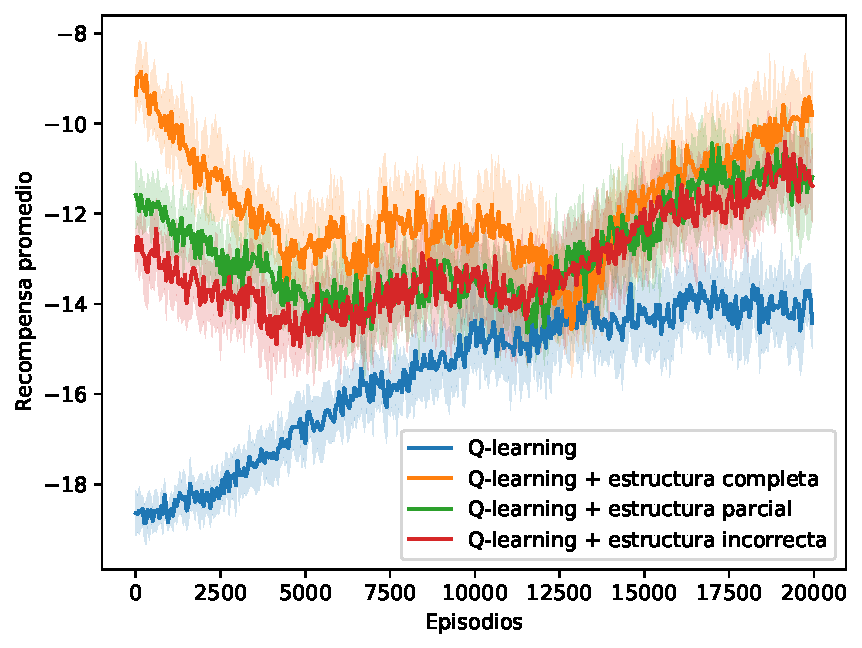
\includegraphics[width=.32\linewidth]{Chapter5/Figs/modexp/stochastic_low_025_one_to_one_N_9_experiments_10_episodes_20000_eps_90000.pdf}&
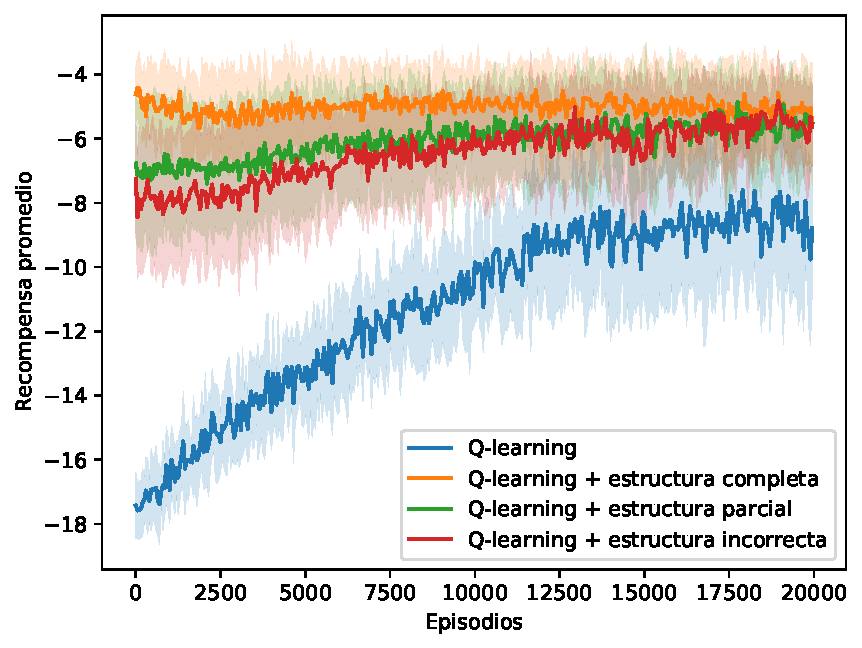
\includegraphics[width=.32\linewidth]{Chapter5/Figs/modexp/stochastic_low_025_one_to_many_N_9_experiments_10_episodes_20000_eps_90000.pdf}&
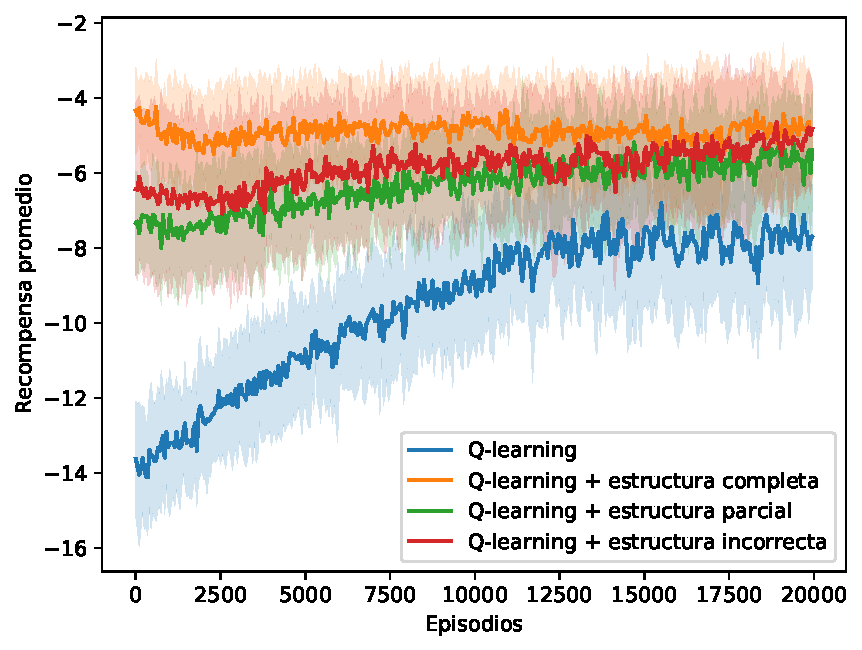
\includegraphics[width=.32\linewidth]{Chapter5/Figs/modexp/stochastic_low_025_many_to_one_N_9_experiments_10_episodes_20000_eps_90000.pdf}

\end{tabular}
\caption{Comparación del desempeño para los 4 algoritmos con un nivel de alteración $p_{mod} = 25 \%$ en un ambiente estocástico. Las gráficas muestran la medida $average$ y la desviación estándar (región sombreada) para 10 experimentos con 10000 (para $N = 5, 7$) y 20000 (para $N = 9$) episodios.}
\label{fig:low-mod-sto}
\end{figure}


\begin{figure}
\settoheight{\tempdima}{\includegraphics[width=.32\linewidth]{example-image-a}}%
\centering\begin{tabular}{@{}c@{ }c@{ }c@{ }c@{}}
&\textbf{Uno-a-uno} & \textbf{Causa común} & \textbf{Efecto común} \\
\rowname{$N = 5$}&
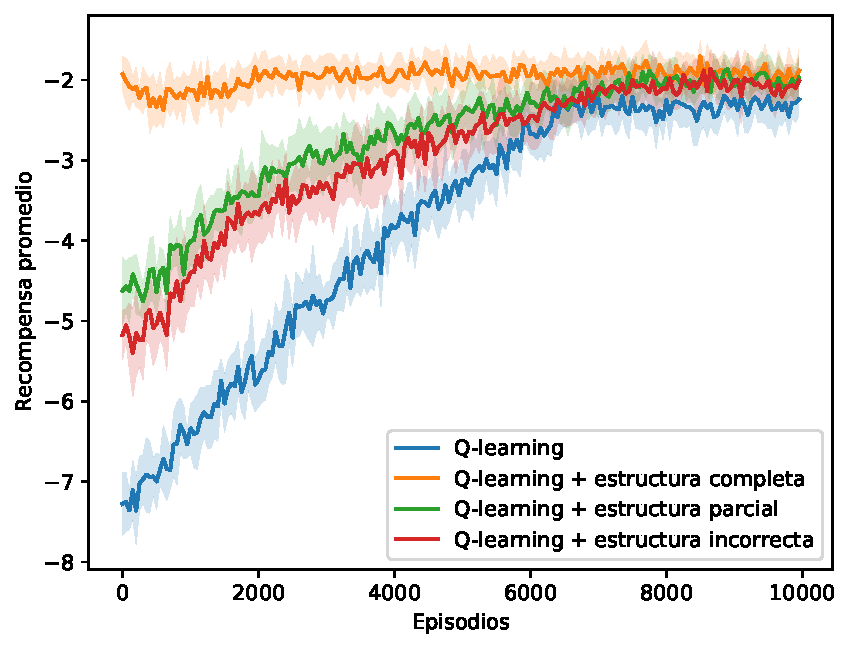
\includegraphics[width=.32\linewidth]{Chapter5/Figs/modexp/deterministic_medium_05_one_to_one_N_5_experiments_10_episodes_10000_eps_25000.pdf}&
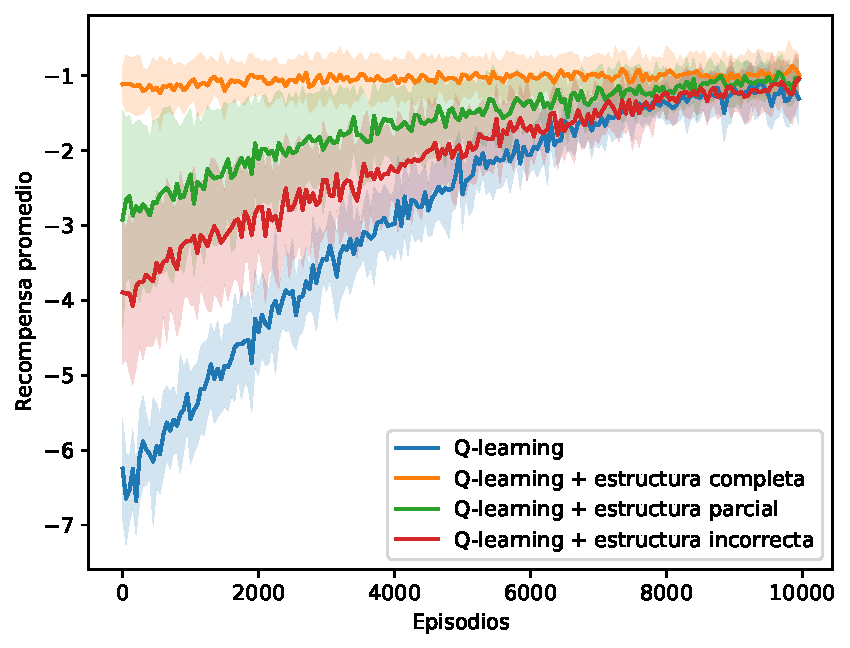
\includegraphics[width=.32\linewidth]{Chapter5/Figs/modexp/deterministic_medium_05_one_to_many_N_5_experiments_10_episodes_10000_eps_25000.pdf}&
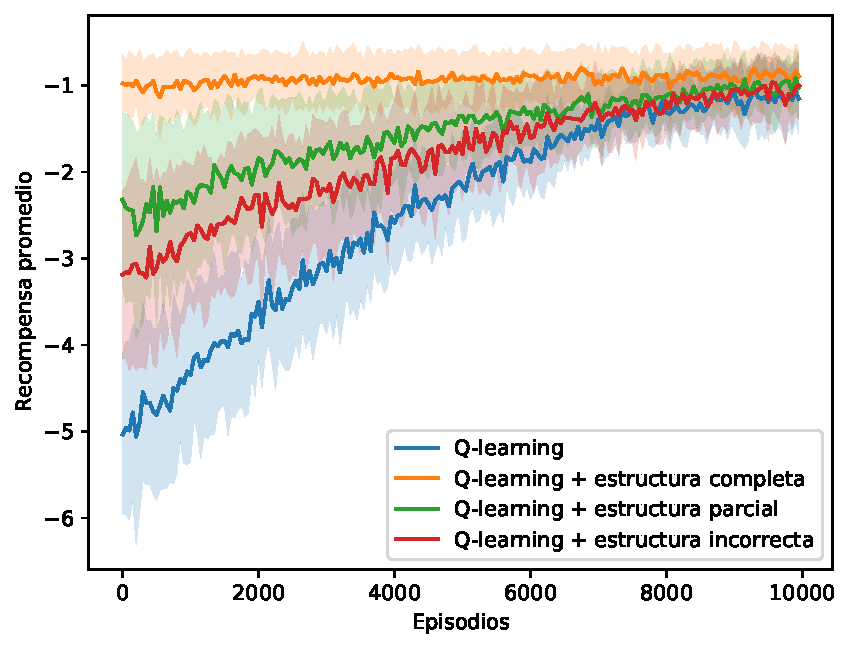
\includegraphics[width=.32\linewidth]{Chapter5/Figs/modexp/deterministic_medium_05_many_to_one_N_5_experiments_10_episodes_10000_eps_25000.pdf}
\\
\rowname{$N=7$}&
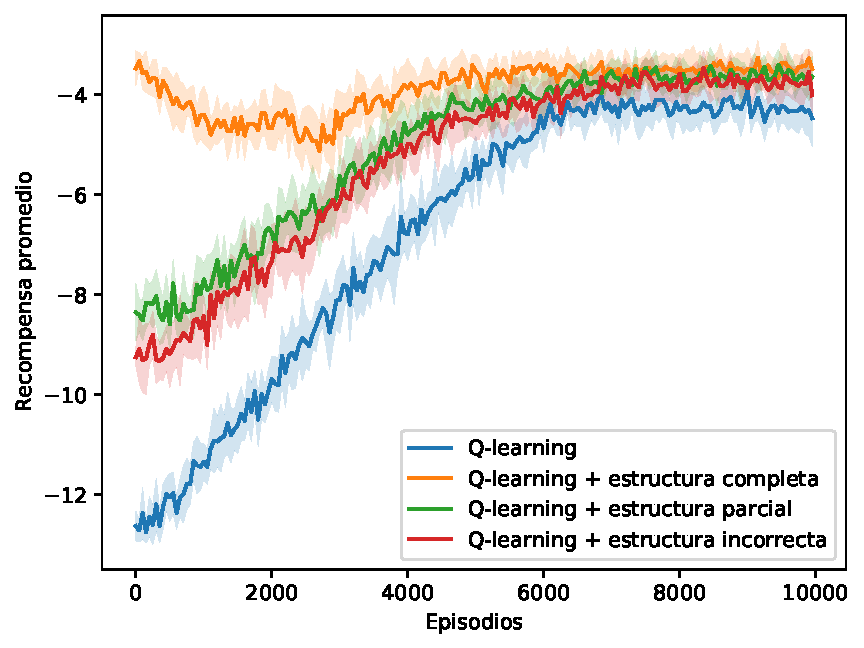
\includegraphics[width=.32\linewidth]{Chapter5/Figs/modexp/deterministic_medium_05_one_to_one_N_7_experiments_10_episodes_10000_eps_35000.pdf}&
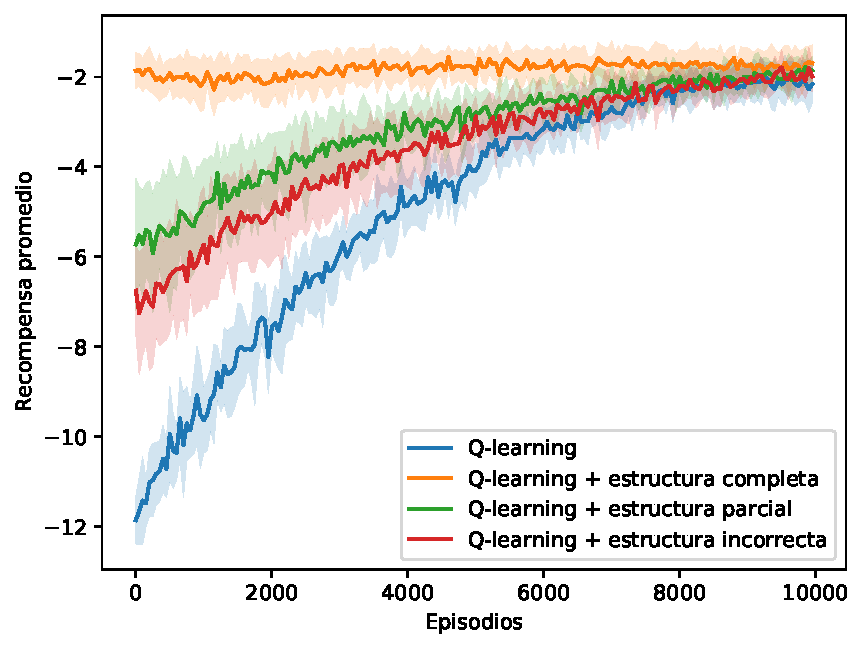
\includegraphics[width=.32\linewidth]{Chapter5/Figs/modexp/deterministic_medium_05_one_to_many_N_7_experiments_10_episodes_10000_eps_35000.pdf}&
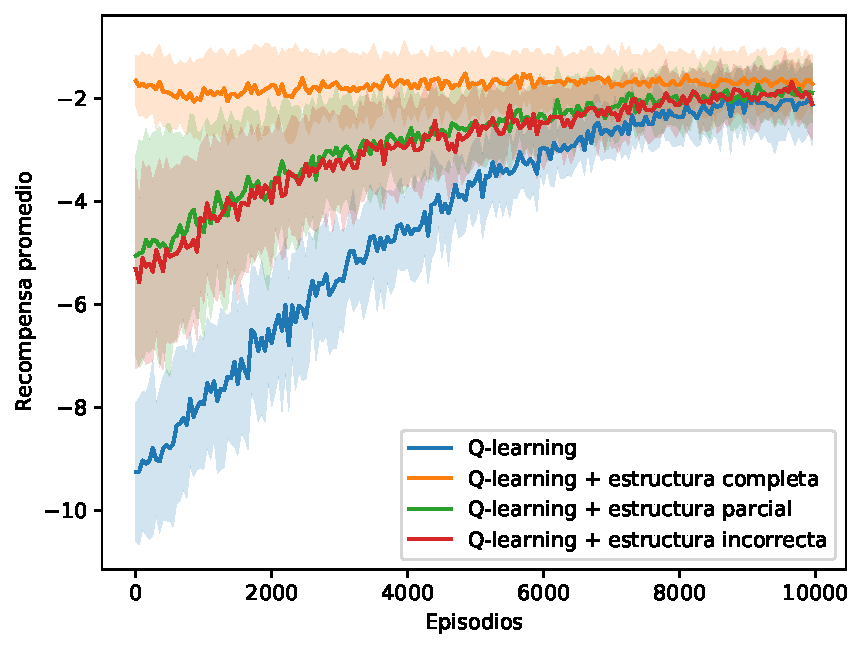
\includegraphics[width=.32\linewidth]{Chapter5/Figs/modexp/deterministic_medium_05_many_to_one_N_7_experiments_10_episodes_10000_eps_35000.pdf}
\\
\rowname{$N = 9$}&

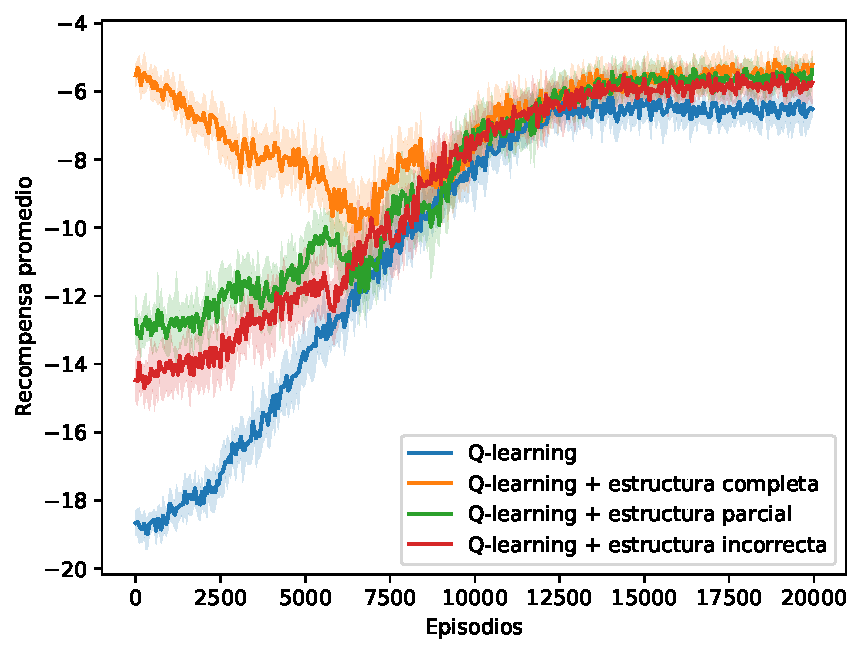
\includegraphics[width=.32\linewidth]{Chapter5/Figs/modexp/deterministic_medium_05_one_to_one_N_9_experiments_10_episodes_20000_eps_90000.pdf}&
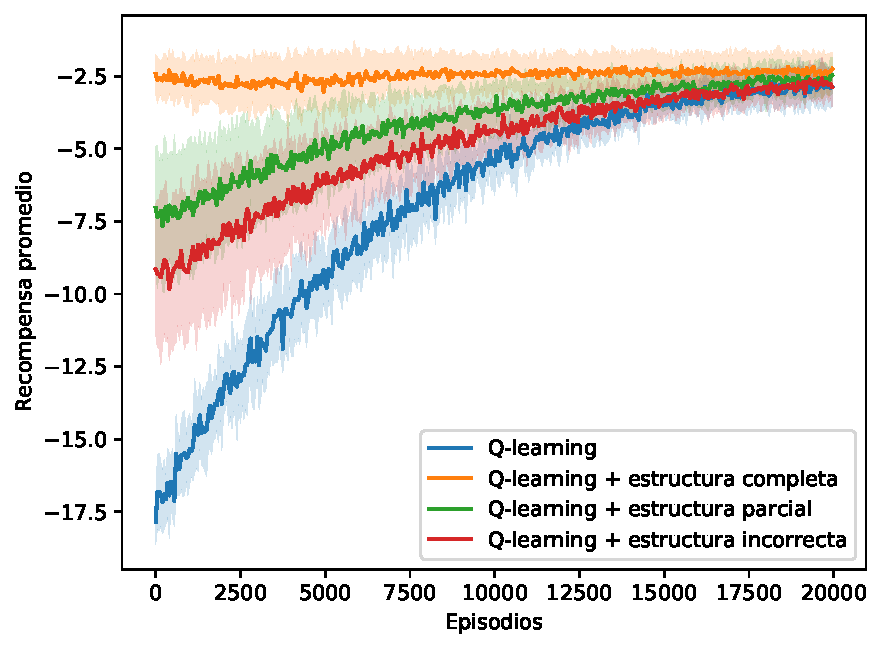
\includegraphics[width=.32\linewidth]{Chapter5/Figs/modexp/deterministic_medium_05_one_to_many_N_9_experiments_10_episodes_20000_eps_90000.pdf}&
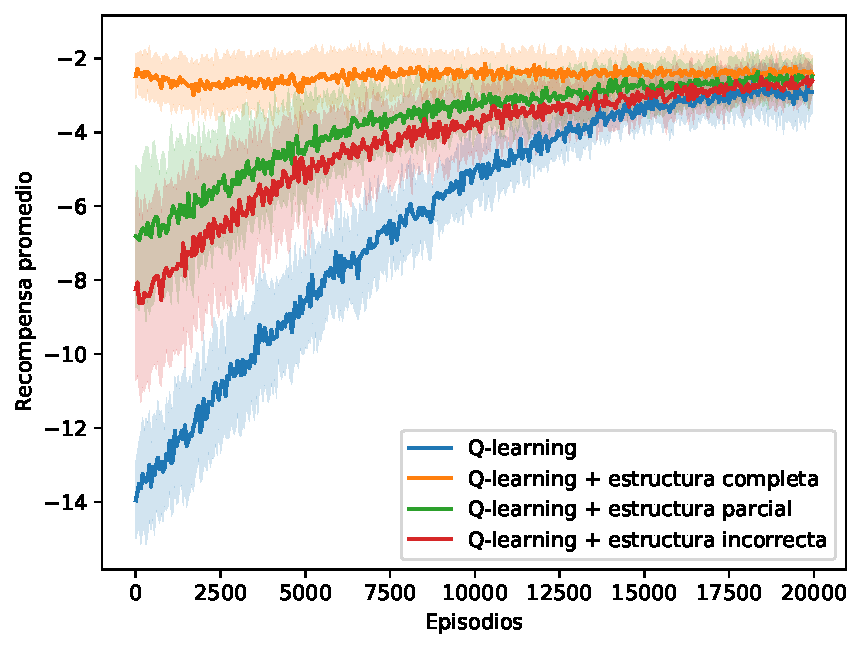
\includegraphics[width=.32\linewidth]{Chapter5/Figs/modexp/deterministic_medium_05_many_to_one_N_9_experiments_10_episodes_20000_eps_90000.pdf}

\end{tabular}
\caption{Comparación del desempeño para los 4 algoritmos con un nivel de alteración $p_{mod} = 50 \%$ en un ambiente determinista. Las gráficas muestran la medida $average$ y la desviación estándar (región sombreada)para 10 experimentos con 10000 (para $N = 5, 7$) y 20000 (para $N = 9$) episodios.}
\label{fig:med-mod-det}
\end{figure}



\begin{figure}
\settoheight{\tempdima}{\includegraphics[width=.32\linewidth]{example-image-a}}%
\centering\begin{tabular}{@{}c@{ }c@{ }c@{ }c@{}}
&\textbf{Uno-a-uno} & \textbf{Causa común} & \textbf{Efecto común} \\
\rowname{$N = 5$}&
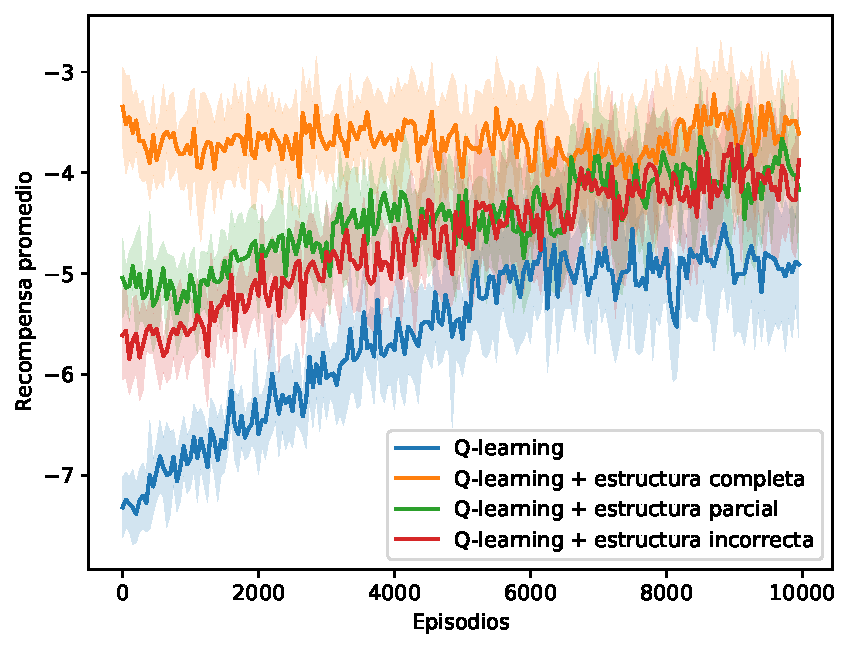
\includegraphics[width=.32\linewidth]{Chapter5/Figs/modexp/stochastic_medium_05_one_to_one_N_5_experiments_10_episodes_10000_eps_25000.pdf}&
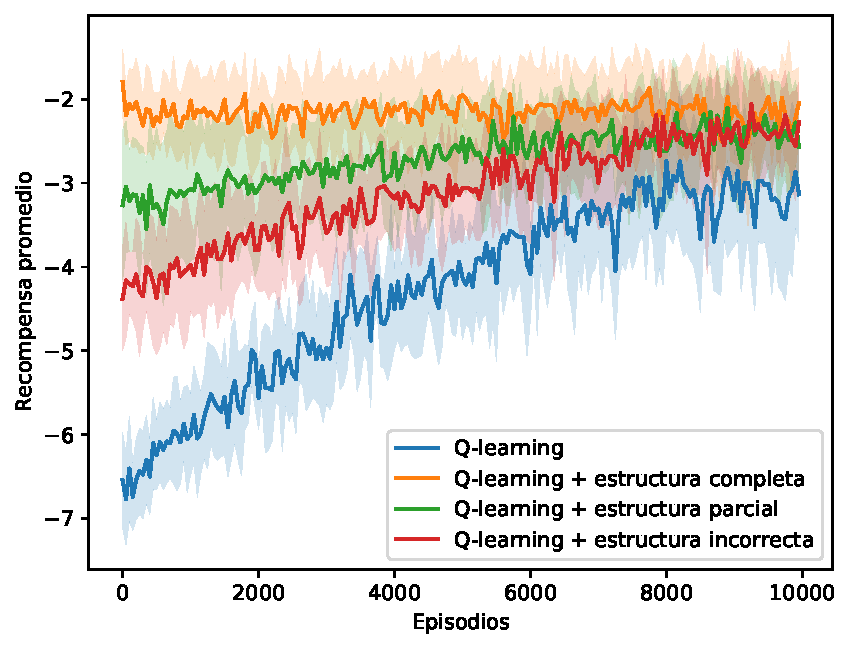
\includegraphics[width=.32\linewidth]{Chapter5/Figs/modexp/stochastic_medium_05_one_to_many_N_5_experiments_10_episodes_10000_eps_25000.pdf}&
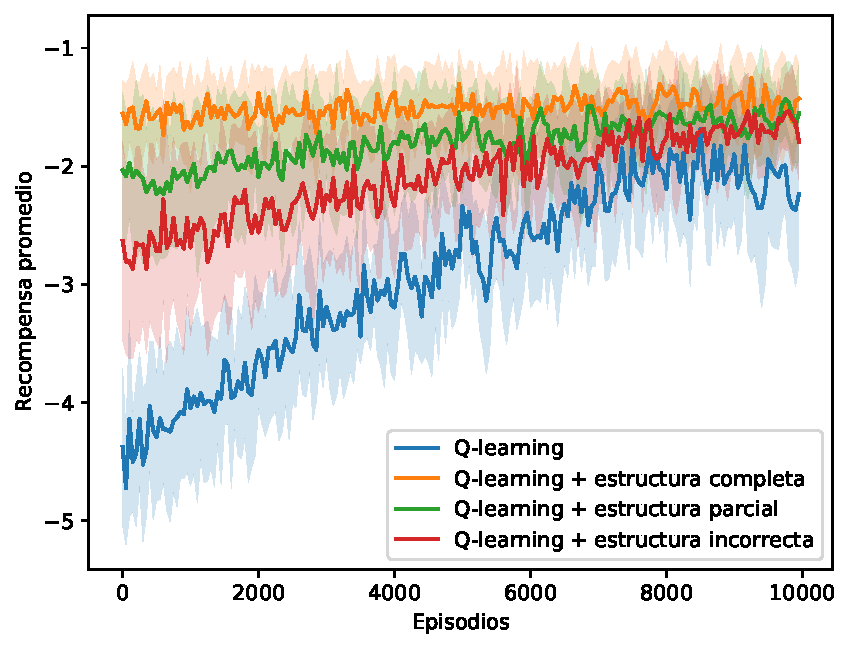
\includegraphics[width=.32\linewidth]{Chapter5/Figs/modexp/stochastic_medium_05_many_to_one_N_5_experiments_10_episodes_10000_eps_25000.pdf}
\\
\rowname{$N=7$}&
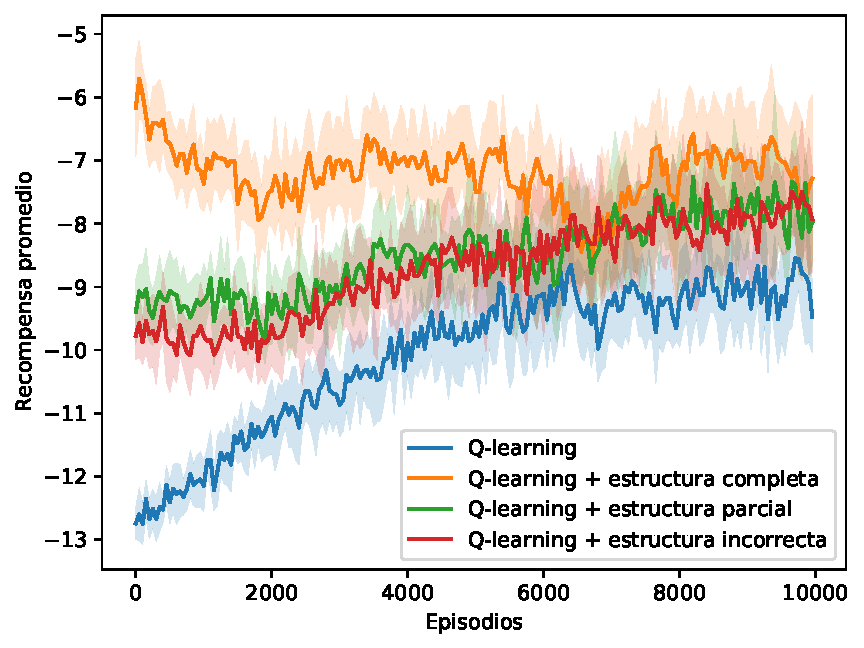
\includegraphics[width=.32\linewidth]{Chapter5/Figs/modexp/stochastic_medium_05_one_to_one_N_7_experiments_10_episodes_10000_eps_35000.pdf}&
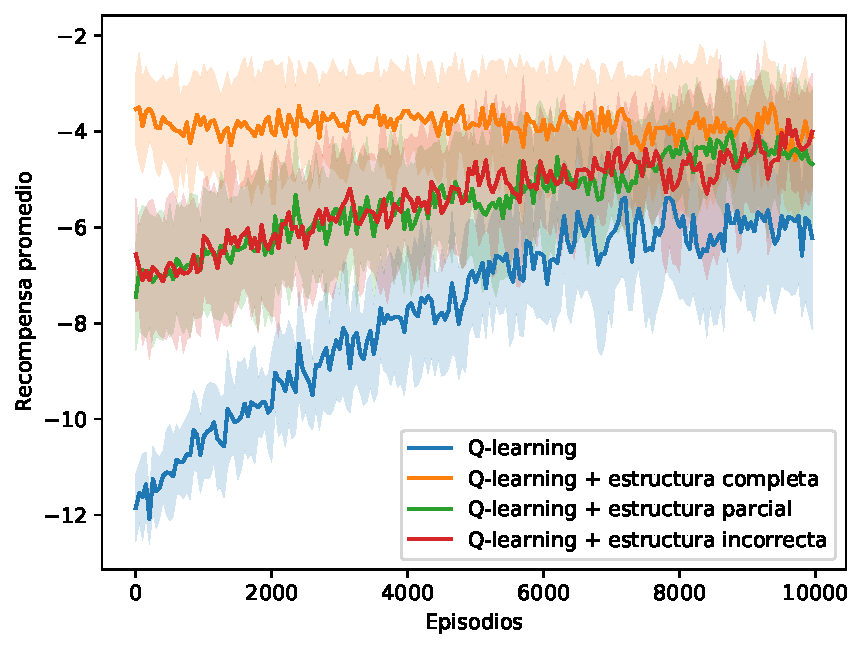
\includegraphics[width=.32\linewidth]{Chapter5/Figs/modexp/stochastic_medium_05_one_to_many_N_7_experiments_10_episodes_10000_eps_35000.pdf}&
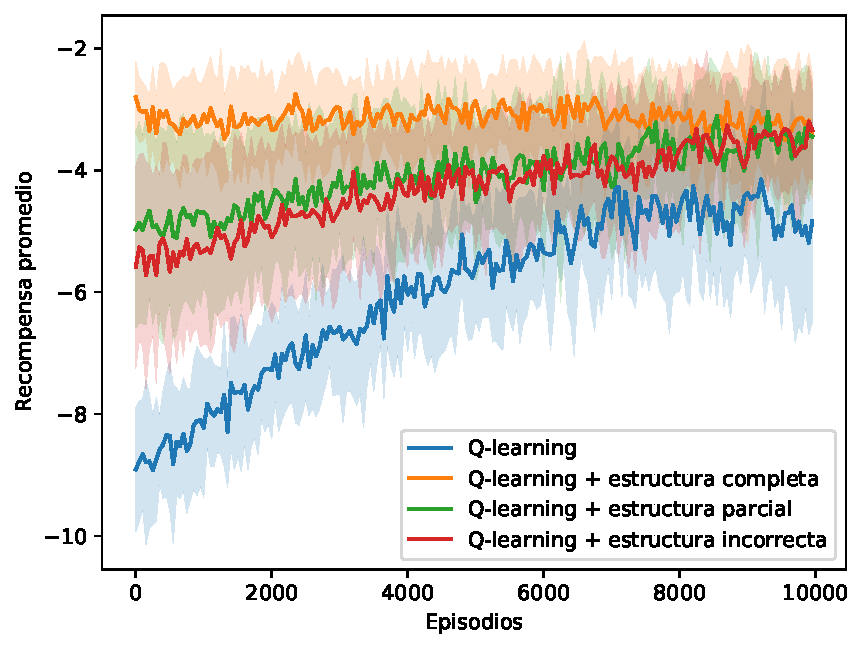
\includegraphics[width=.32\linewidth]{Chapter5/Figs/modexp/stochastic_medium_05_many_to_one_N_7_experiments_10_episodes_10000_eps_35000.pdf}
\\
\rowname{$N = 9$}&

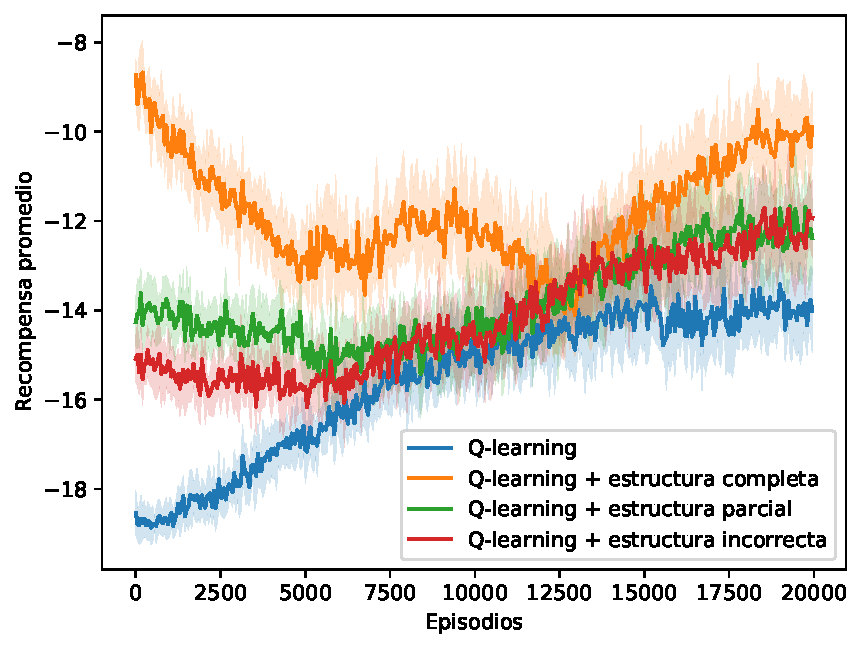
\includegraphics[width=.32\linewidth]{Chapter5/Figs/modexp/stochastic_medium_05_one_to_one_N_9_experiments_10_episodes_20000_eps_90000.pdf}&
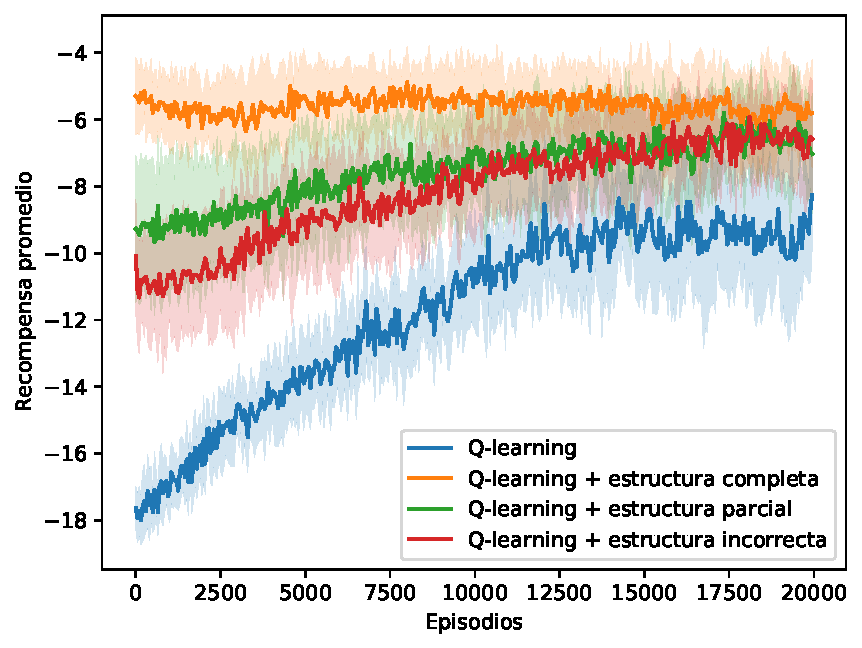
\includegraphics[width=.32\linewidth]{Chapter5/Figs/modexp/stochastic_medium_05_one_to_many_N_9_experiments_10_episodes_20000_eps_90000.pdf}&
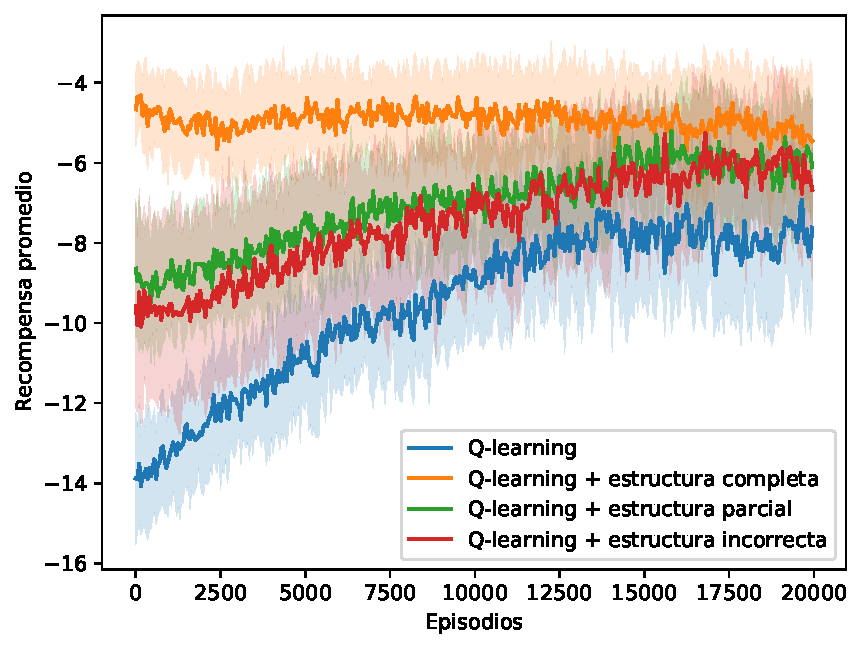
\includegraphics[width=.32\linewidth]{Chapter5/Figs/modexp/stochastic_medium_05_many_to_one_N_9_experiments_10_episodes_20000_eps_90000.pdf}

\end{tabular}
\caption{Comparación del desempeño para los 4 algoritmos con un nivel de alteración $p_{mod} = 50 \%$ en un ambiente estocástico. Las gráficas muestran la medida $average$ y la desviación estándar (región sombreada)para 10 experimentos con 10000 (para $N = 5, 7$) y 20000 (para $N = 9$) episodios.}
\label{fig:med-mod-sto}
\end{figure}



\begin{figure}
\settoheight{\tempdima}{\includegraphics[width=.32\linewidth]{example-image-a}}%
\centering\begin{tabular}{@{}c@{ }c@{ }c@{ }c@{}}
&\textbf{Uno-a-uno} & \textbf{Causa común} & \textbf{Efecto común} \\
\rowname{$N = 5$}&
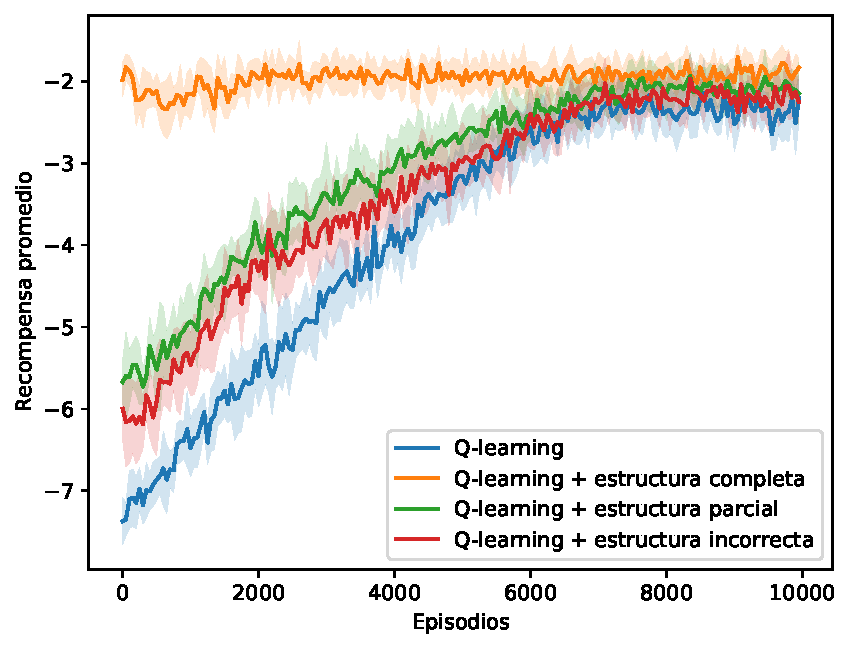
\includegraphics[width=.32\linewidth]{Chapter5/Figs/modexp/deterministic_high_075_one_to_one_N_5_experiments_10_episodes_10000_eps_25000.pdf}&
\includegraphics[width=.32\linewidth]{Chapter5/Figs/modexp/deterministic_high_075_one_to_many_N_5_experiments_10_episodes_10000_eps_25000.pdf}&
\includegraphics[width=.32\linewidth]{Chapter5/Figs/modexp/deterministic_high_075_many_to_one_N_5_experiments_10_episodes_10000_eps_25000.pdf}
\\
\rowname{$N=7$}&
\includegraphics[width=.32\linewidth]{Chapter5/Figs/modexp/deterministic_high_075_one_to_one_N_7_experiments_10_episodes_10000_eps_35000.pdf}&
\includegraphics[width=.32\linewidth]{Chapter5/Figs/modexp/deterministic_high_075_one_to_many_N_7_experiments_10_episodes_10000_eps_35000.pdf}&
\includegraphics[width=.32\linewidth]{Chapter5/Figs/modexp/deterministic_high_075_many_to_one_N_7_experiments_10_episodes_10000_eps_35000.pdf}
\\
\rowname{$N = 9$}&

\includegraphics[width=.32\linewidth]{Chapter5/Figs/modexp/deterministic_high_075_one_to_one_N_9_experiments_10_episodes_20000_eps_90000.pdf}&
\includegraphics[width=.32\linewidth]{Chapter5/Figs/modexp/deterministic_high_075_one_to_many_N_9_experiments_10_episodes_20000_eps_90000.pdf}&
\includegraphics[width=.32\linewidth]{Chapter5/Figs/modexp/deterministic_high_075_many_to_one_N_9_experiments_10_episodes_20000_eps_90000.pdf}


\end{tabular}

\caption{Comparación del desempeño para los 4 algoritmos con un nivel de alteración $p_{mod} = 75 \%$ en un ambiente determinista. Las gráficas muestran la medida $average$ y la desviación estándar (región sombreada) para 10 experimentos con 10000 (para $N = 5, 7$) y 20000 (para $N = 9$) episodios.}
\label{fig:high-mod-det}
\end{figure}

\begin{figure}
\settoheight{\tempdima}{\includegraphics[width=.32\linewidth]{example-image-a}}%
\centering\begin{tabular}{@{}c@{ }c@{ }c@{ }c@{}}
&\textbf{Uno-a-uno} & \textbf{Causa común} & \textbf{Efecto común} \\
\rowname{$N = 5$}&
\includegraphics[width=.32\linewidth]{Chapter5/Figs/modexp/stochastic_high_075_one_to_one_N_5_experiments_10_episodes_10000_eps_25000.pdf}&
\includegraphics[width=.32\linewidth]{Chapter5/Figs/modexp/stochastic_high_075_one_to_many_N_5_experiments_10_episodes_10000_eps_25000.pdf}&
\includegraphics[width=.32\linewidth]{Chapter5/Figs/modexp/stochastic_high_075_many_to_one_N_5_experiments_10_episodes_10000_eps_25000.pdf}
\\
\rowname{$N=7$}&
\includegraphics[width=.32\linewidth]{Chapter5/Figs/modexp/stochastic_high_075_one_to_one_N_7_experiments_10_episodes_10000_eps_35000.pdf}&
\includegraphics[width=.32\linewidth]{Chapter5/Figs/modexp/stochastic_high_075_one_to_many_N_7_experiments_10_episodes_10000_eps_35000.pdf}&
\includegraphics[width=.32\linewidth]{Chapter5/Figs/modexp/stochastic_high_075_many_to_one_N_7_experiments_10_episodes_10000_eps_35000.pdf}
\\
\rowname{$N = 9$}&

\includegraphics[width=.32\linewidth]{Chapter5/Figs/modexp/stochastic_high_075_one_to_one_N_9_experiments_10_episodes_20000_eps_90000.pdf}&
\includegraphics[width=.32\linewidth]{Chapter5/Figs/modexp/stochastic_high_075_one_to_many_N_9_experiments_10_episodes_20000_eps_90000.pdf}&
\includegraphics[width=.32\linewidth]{Chapter5/Figs/modexp/stochastic_high_075_many_to_one_N_9_experiments_10_episodes_20000_eps_90000.pdf}
\end{tabular}

\caption{Comparación del desempeño para los 4 algoritmos con un nivel de alteración $p_{mod} = 75 \%$ en un ambiente estocástico. Las gráficas muestran la medida $average$ y la desviación estándar (región sombreada) para 10 experimentos con 10000 (para $N = 5, 7$) y 20000 (para $N = 9$) episodios.}
\label{fig:high-mod-sto}
\end{figure}



\clearpage

\subsection{Explotar o seguir explorando}\label{subsection:exp-epsilon}

En esta sección se muestran los experimentos para comparar
el desempeño de los algoritmos con dos valores diferentes para
el factor que controla la tasa de decremento de $\epsilon$. El primer valor 
es bajo, para dejar de dar peso a la exploración después del primer
cuarto de entrenamiento y el segundo es alto, para llegar a una máxima probabilidad
de explotación en el último cuarto del aprendizaje.

\subsubsection{Configuración experimental}

\begin{itemize}
    \item El espacio de estados es discreto, es decir, el agente puede
    obtener las variables $\mathcal{X}$ directamente del ambiente.
    \item Para obtener a los
    grafos $\mathcal{D'}$ y $\mathcal{D''}$,
    el porcentaje de nivel de cambio  es $p_{mod} = 25 \%$. Esto significa que no se altera demasiado el grafo causal original para
    generar los grafos incompletos e incorrectos.
    \item Se controla qué tan rápido se desea alcanzar $\epsilon_{\min}$ variando el parámetro $\delta$. Si se divide al entrenamiento en cuartos,  entonces los valores de $\delta$ corresponden a en qué cuarto se alcanza el mínimo valor para $\epsilon$.
    \begin{itemize}
        \item Alcanzar $\epsilon_{\min}$ en el primer cuarto del entrenamiento, $\delta = 0.25$.
        \item Alcanzar $\epsilon_{\min}$ a medio aprendizaje, $\delta = 0.50$.
        \item Alcanzar $\epsilon_{\min}$ en el tercer cuarto del entrenamiento, $\delta = 0.75$.
    \end{itemize}
    \item Se examina sobre los tres tipos de estructuras posibles: uno-a-uno, 
    causa común y efecto común. 
    \item Se prueba sobre un mundo determinista y uno estocástico.
    \item Dado que en la sección \ref{exp1}, $\delta=0.5$, este valor se deja fuera para estos experimentos.
\end{itemize}

\subsubsection{Objetivo}

Determinar si reducir o aumentar las consultas al grafo causal a lo largo del aprendizaje afecta el desempeño
de los algoritmos.

\subsubsection{Hipótesis}

La información del grafo causal no afecta negativamente 
el aprendizaje de la función de valor $Q$. Por lo tanto, incluso si se disminuyen las consultas al modelo de manera temprana en el entrenamiento, la información provista habrá
ayudado al aprendizaje de la función de valor.

\subsubsection{Resultados}

A fin de  comparar el desempeño de los algoritmos
para las diferentes configuraciones del experimento
se evalúa la medida \textit{average}.
De manera gráfica, se muestra el desempeño de los algoritmos
para los diferentes valores $\delta$ en las Figuras \ref{fig:low-epsilon-det}, \ref{fig:low-epsilon-sto}, \ref{fig:high-epsilon-det} y \ref{fig:high-epsilon-sto}.

En las Figuras \ref{fig:low-epsilon-det}-\ref{fig:high-epsilon-sto} se puede ver que en la mayoría de los casos, los algoritmos que utilizan conocimiento del grafo inician con una recompensa mayor y se estabilizan más rápido que el algoritmo Q-learning
sin información adicional en ambientes con transiciones deterministas y estocásticas.
De acuerdo con los resultados parece que 
entre mayor sea $\delta$ más tarda en estabilizarse
el algoritmo de aprendizaje sin información que lo auxilie. Esto es de esperarse, ya que se sigue explorando durante más tiempo. 
Por otro lado, para las estructuras uno-a-uno, la recompensa en los algoritmos que se guían por el grafo, se desestabiliza el intervalo en el que se encuentra la transición a dejar de dar peso a
la exploración. Pero, una vez fuera de esa ``zona de transición'' los
algoritmos se recuperan y tienden a estar por encima del algoritmo sin datos 
extra.

Por otro lado, además de las curvas de aprendizaje se propone hacer una comparación estadística de
los métodos. Para esto, se
compara la recompensa promedio de los últimos $E$ episodios
de entrenamiento sobre los $M$ experimentos. Con esto, se 
puede obtener una muestra de tamaño $E$ para cada algoritmo
y hacer una prueba estadística para mostrar que existe una diferencia entre ellos. La prueba estadística se realiza comparando los algoritmos que utilizan información extra versus el algoritmo Q-learning usando una exploración a prueba y error para saber si los primeros son superiores significativamente sobre el segundo. 

En las tablas \ref{tab:delta-one-to-one}, \ref{tab:delta-one-to-many} y \ref{tab:delta-many-to-one} se muestran
los promedios de las recompensas durante los últimos $E$ episodios. 
De igual manera que en las curvas de aprendizaje se puede notar que en la mayoría de tareas el algoritmo Q-learning usando el grafo causal completo tiene una recompensa mayor que en los otros métodos. Además, en general los métodos que utilizan el grafo ya sea incorrecto o incompleto superan al método clásico de Q-learning. Para validar estos resultados se usa la prueba de Welch con $p < 0.05$ para encontrar diferencias estadísticamente significativas. 
Los resultados de las pruebas refuerzan lo concluido a partir de las gráficas. Existe una diferencia estadística en el desempeño de los algoritmos, excepto por algunos casos (marcados por $\dagger$ en las tablas). Estos últimos corresponden
al desempeño en tareas con una estructura causal subyacente de tipo uno a uno y con $N=9$. Esto puede ser debido a esta transición
de exploración y explotación. 

\begin{table}[h]
\centering
\caption{Comparación de la recompensa promedio obtenida durante los últimos $E=100$ episodios de entrenamiento para $M$ experimentos en tareas con estructuras causales uno a uno. En negritas se resaltan las recompensas promedio mayores con respecto al resto de los algoritmos en una configuración experimental dada.}
\label{tab:delta-one-to-one}
\resizebox{\textwidth}{!}{%
\begin{tabular}{@{}ccclll@{}}
\toprule
Ambiente & $\delta$ & Algoritmo & \multicolumn{3}{c}{$N$} \\ \cmidrule(l){4-6} 
 &  &  & \multicolumn{1}{c}{5} & \multicolumn{1}{c}{7} & \multicolumn{1}{c}{9} \\ \midrule
Determinista & $0.25$ & $Q_{1}$ & $-2.2324 \pm 0.6353$ & $-4.3184 \pm 0.8746$ & $-6.3564 \pm 1.3603$ \\
 &  & $Q_{2}$ & $\mathbf{-1.9466 \pm 0.4679}$ & $-3.5731 \pm 0.7285$ & $-5.7115 \pm 1.1855$ \\
 &  & $Q_{2}$ & $-1.9825 \pm 0.4632$ & $\mathbf{-3.5061 \pm 0.7207}$ & $\mathbf{-5.6209 \pm 1.0718}$ \\
 &  & $Q_{4}$ & $-2.0330 \pm 0.5384$ & $-3.5547 \pm 0.7081$ & $-5.8372 \pm 1.0747$ \\ \cmidrule(l){2-6} 
 & $0.75$ & $Q_{1}$ & $-2.3774 \pm 0.6925$ & $-4.3218 \pm 0.9312$ & $-6.2775 \pm 1.1195$ \\
 &  & $Q_{2}$ & $\mathbf{-1.8880 \pm 0.4666}$ & $\mathbf{-3.4929 \pm 0.7115}$ & $-6.9414 \pm 1.6493$ \\
 &  & $Q_{2}$ & $-2.1314 \pm 0.4933$ & $-3.8299 \pm 0.7694$ & $-6.3671 \pm 1.4099\dagger$ \\
 &  & $Q_{4}$ & $-1.9896 \pm 0.5470$ & $-3.8252 \pm 0.7840$ & $\mathbf{-6.2538 \pm 1.3547\dagger}$ \\ \cmidrule(l){2-6} 
Estocástico & $0.25$ & $Q_{1}$ & $-4.8575 \pm 0.9453$ & $-9.3174 \pm 1.2780$ & $-14.5087 \pm 1.4934$ \\
 &  & $Q_{2}$ & $\mathbf{-3.4833 \pm 0.8100}$ & $-7.2904 \pm 1.3719$ & $\mathbf{-10.7682 \pm 1.8282}$ \\
 &  & $Q_{2}$ & $-3.7870 \pm 0.8263$ & $\mathbf{-6.8757 \pm 1.2246}$ & $-11.9817 \pm 1.9420$ \\
 &  & $Q_{4}$ & $-3.8850 \pm 0.8119$ & $-7.1184 \pm 1.1471$ & $-12.4496 \pm 1.9692$ \\ \cmidrule(l){2-6} 
 & $0.75$ & $Q_{1}$ & $-5.0956 \pm 0.8950$ & $-9.3535 \pm 1.2484$ & $-14.3432 \pm 1.7236$ \\
 &  & $Q_{2}$ & $\mathbf{-3.9598 \pm 0.8291}$ & $-8.1395 \pm 1.3979$ & $\mathbf{-13.7784 \pm 1.8453}$ \\
 &  & $Q_{2}$ & $-4.2412 \pm 0.9166$ & $-8.4381 \pm 1.4981$ & $-13.8170 \pm 2.0379\dagger$ \\
 &  & $Q_{4}$ & $-3.9809 \pm 0.8148$ & $\mathbf{-8.1071 \pm 1.2102}$ & $-13.9492 \pm 1.7832\dagger$ \\ \bottomrule
\end{tabular}%
}
\end{table}

\newpage

\begin{table}[]
\centering
\caption{Comparación de la recompensa promedio obtenida durante los últimos $E=100$ episodios de entrenamiento para $M$ experimentos en tareas con estructuras de causa común. En negritas se resaltan las recompensas promedio mayores con respecto al resto de los algoritmos en una configuración experimental dada.}
\label{tab:delta-one-to-many}
\resizebox{\textwidth}{!}{%
\begin{tabular}{ccclll}
\hline
Ambiente & $\delta$ & Algoritmo & \multicolumn{3}{c}{$N$} \\ \cline{4-6} 
 &  &  & \multicolumn{1}{c}{5} & \multicolumn{1}{c}{7} & \multicolumn{1}{c}{9} \\ \hline
Determinista & $0.25$ & $Q_{1}$ & $-1.1242 \pm 0.4301$ & $-2.4038 \pm 0.7038$ & $-2.9975 \pm 0.8161$ \\
 &  & $Q_{2}$ & $-0.8281 \pm 0.2998$ & $\mathbf{-1.8221 \pm 0.5187}$ & $\mathbf{-2.4173 \pm 0.5790}$ \\
 &  & $Q_{2}$ & $-0.8161 \pm 0.2827$ & $-1.8789 \pm 0.4548$ & $-2.5532 \pm 0.5628$ \\
 &  & $Q_{4}$ & $\mathbf{-0.8068 \pm 0.3186}$ & $-1.8897 \pm 0.4411$ & $-2.5236 \pm 0.6685$ \\ \cline{2-6} 
 & $0.75$ & $Q_{1}$ & $-1.6430 \pm 0.6236$ & $-2.9379 \pm 0.7767$ & $-4.1146 \pm 1.2066$ \\
 &  & $Q_{2}$ & $\mathbf{-0.9273 \pm 0.2693}$ & $\mathbf{-1.6828 \pm 0.4610}$ & $\mathbf{-2.6278 \pm 0.6338}$ \\
 &  & $Q_{2}$ & $-1.0958 \pm 0.4066$ & $-1.9402 \pm 0.6138$ & $-2.9660 \pm 0.6821$ \\
 &  & $Q_{4}$ & $-1.0778 \pm 0.3990$ & $-1.9267 \pm 0.5551$ & $-3.3222 \pm 0.8773$ \\ \cline{2-6} 
Estocástico & $0.25$ & $Q_{1}$ & $-2.8257 \pm 0.8804$ & $-6.0498 \pm 1.4224$ & $-8.9472 \pm 1.7429$ \\
 &  & $Q_{2}$ & $\mathbf{-2.1866 \pm 0.7467}$ & $\mathbf{-4.0352 \pm 1.0788}$ & $\mathbf{-5.0238 \pm 1.3692}$ \\
 &  & $Q_{2}$ & $-2.2934 \pm 0.7969$ & $-4.0734 \pm 1.2090$ & $-5.3714 \pm 1.4905$ \\
 &  & $Q_{4}$ & $-2.2001 \pm 0.7131$ & $-4.2083 \pm 1.1122$ & $-5.4152 \pm 1.5542$ \\ \cline{2-6} 
 & $0.75$ & $Q_{1}$ & $-3.3176 \pm 1.0664$ & $-6.3604 \pm 1.4621$ & $-9.7091 \pm 1.8713$ \\
 &  & $Q_{2}$ & $\mathbf{-2.0068 \pm 0.6758}$ & $\mathbf{-4.1851 \pm 1.0592}$ & $\mathbf{-5.7100 \pm 1.5696}$ \\
 &  & $Q_{2}$ & $-2.2042 \pm 0.7600$ & $-4.5311 \pm 1.2282$ & $-6.8496 \pm 1.5566$ \\
 &  & $Q_{4}$ & $-2.3583 \pm 0.7962$ & $-4.6244 \pm 1.2486$ & $-6.3323 \pm 1.6861$ \\ \hline
\end{tabular}%
}
\end{table}

\begin{table}[]
\centering
\caption{Comparación de la recompensa promedio obtenida durante los últimos $E=100$ episodios de entrenamiento para $M$ experimentos en tareas con estructuras con relaciones de efecto común. En negritas se resaltan las recompensas promedio mayores con respecto al resto de los algoritmos en una configuración experimental dada.}
\label{tab:delta-many-to-one}
\resizebox{\textwidth}{!}{%
\begin{tabular}{ccclll}
\hline
Ambiente & $\delta$ & Algoritmo & \multicolumn{3}{c}{$N$} \\ \cline{4-6} 
 &  &  & \multicolumn{1}{c}{5} & \multicolumn{1}{c}{7} & \multicolumn{1}{c}{9} \\ \hline
Determinista & $0.25$ & $Q_{1}$ & $-0.9308 \pm 0.3887$ & $-2.0693 \pm 0.6689$ & $-2.9613 \pm 0.7537$ \\
 &  & $Q_{2}$ & $\mathbf{-0.6354 \pm 0.2388}$ & $\mathbf{-1.5994 \pm 0.4242}$ & $-2.5653 \pm 0.5053$ \\
 &  & $Q_{2}$ & $-0.7521 \pm 0.2444$ & $-1.6121 \pm 0.4051$ & $\mathbf{-2.5128 \pm 0.5890}$ \\
 &  & $Q_{4}$ & $-0.6659 \pm 0.2323$ & $-1.5995 \pm 0.4407$ & $-2.6478 \pm 0.6228$ \\ \cline{2-6} 
 & $0.75$ & $Q_{1}$ & $-1.5390 \pm 0.5056$ & $-2.9007 \pm 0.7137$ & $-3.9921 \pm 1.0301$ \\
 &  & $Q_{2}$ & $\mathbf{-0.8006 \pm 0.2368}$ & $\mathbf{-1.7237 \pm 0.4467}$ & $\mathbf{-2.4808 \pm 0.5215}$ \\
 &  & $Q_{2}$ & $-0.9448 \pm 0.3327$ & $-1.9036 \pm 0.5026$ & $-2.8287 \pm 0.7198$ \\
 &  & $Q_{4}$ & $-0.8983 \pm 0.3522$ & $-1.7377 \pm 0.4231$ & $-2.9039 \pm 0.7814$ \\ \cline{2-6} 
Estocástico & $0.25$ & $Q_{1}$ & $-2.7417 \pm 0.8380$ & $-5.2262 \pm 1.1446$ & $-7.6755 \pm 1.5417$ \\
 &  & $Q_{2}$ & $-2.0551 \pm 0.6530$ & $-3.6230 \pm 1.0363$ & $\mathbf{-4.4380 \pm 1.1340}$ \\
 &  & $Q_{2}$ & $-2.0618 \pm 0.5730$ & $\mathbf{-3.3963 \pm 0.8821}$ & $-4.7390 \pm 1.1393$ \\
 &  & $Q_{4}$ & $\mathbf{-1.9463 \pm 0.6109}$ & $-3.6499 \pm 1.0723$ & $-5.6039 \pm 1.3790$ \\ \cline{2-6} 
 & $0.75$ & $Q_{1}$ & $-2.7992 \pm 0.8305$ & $-5.6699 \pm 1.3177$ & $-7.7359 \pm 1.7315$ \\
 &  & $Q_{2}$ & $\mathbf{-1.6935 \pm 0.5582}$ & $\mathbf{-3.7668 \pm 1.1628}$ & $\mathbf{-5.0338 \pm 1.0605}$ \\
 &  & $Q_{2}$ & $-1.8176 \pm 0.6096$ & $-4.0601 \pm 1.0350$ & $-5.9173 \pm 1.3811$ \\
 &  & $Q_{4}$ & $-2.2837 \pm 0.6340$ & $-4.5129 \pm 1.0016$ & $-5.6167 \pm 1.5121$ \\ \hline
\end{tabular}%
}
\end{table}

\newpage

\begin{figure}
\settoheight{\tempdima}{\includegraphics[width=.32\linewidth]{example-image-a}}%
\centering\begin{tabular}{@{}c@{ }c@{ }c@{ }c@{}}
&\textbf{Uno-a-uno} & \textbf{Causa común} & \textbf{Efecto común} \\
\rowname{$N = 5$}&
\includegraphics[width=.32\linewidth]{Chapter5/Figs/deltaexp/deterministic_low_025_one_to_one_N_5_experiments_10_episodes_5000_eps_6250.pdf}&
\includegraphics[width=.32\linewidth]{Chapter5/Figs/deltaexp/deterministic_low_025_one_to_many_N_5_experiments_10_episodes_5000_eps_6250.pdf}&
\includegraphics[width=.32\linewidth]{Chapter5/Figs/deltaexp/deterministic_low_025_many_to_one_N_5_experiments_10_episodes_5000_eps_6250.pdf}\\
\rowname{$N=7$}&
\includegraphics[width=.32\linewidth]{Chapter5/Figs/deltaexp/deterministic_low_025_one_to_one_N_7_experiments_10_episodes_5000_eps_8750.pdf}&
\includegraphics[width=.32\linewidth]{Chapter5/Figs/deltaexp/deterministic_low_025_one_to_many_N_7_experiments_10_episodes_5000_eps_8750.pdf}&
\includegraphics[width=.32\linewidth]{Chapter5/Figs/deltaexp/deterministic_low_025_many_to_one_N_7_experiments_10_episodes_5000_eps_8750.pdf}\\
\rowname{$N = 9$}&
\includegraphics[width=.32\linewidth]{Chapter5/Figs/deltaexp/deterministic_low_025_one_to_one_N_9_experiments_10_episodes_10000_eps_22500.pdf}&
\includegraphics[width=.32\linewidth]{Chapter5/Figs/deltaexp/deterministic_low_025_one_to_many_N_9_experiments_10_episodes_10000_eps_22500.pdf}&
\includegraphics[width=.32\linewidth]{Chapter5/Figs/deltaexp/deterministic_low_025_many_to_one_N_9_experiments_10_episodes_10000_eps_22500.pdf}
\end{tabular}
\caption{Comparación del desempeño para los 4 algoritmos con un nivel de alteración $p_{mod} = 25 \%$  y $\delta = 0.25$ en un ambiente determinista. Las gráficas muestran la medida $average$ y la desviación estándar (región sombreada) para 10 experimentos con 5000 (para $N = 5, 7$) y 10000 (para $N = 9$) episodios.}
\label{fig:low-epsilon-det}
\end{figure}

\newpage

\begin{figure}
\settoheight{\tempdima}{\includegraphics[width=.32\linewidth]{example-image-a}}%
\centering\begin{tabular}{@{}c@{ }c@{ }c@{ }c@{}}
&\textbf{Uno-a-uno} & \textbf{Causa común} & \textbf{Efecto común} \\
\rowname{$N = 5$}&
\includegraphics[width=.32\linewidth]{Chapter5/Figs/deltaexp/stochastic_low_025_one_to_one_N_5_experiments_10_episodes_5000_eps_6250.pdf}&
\includegraphics[width=.32\linewidth]{Chapter5/Figs/deltaexp/stochastic_low_025_one_to_many_N_5_experiments_10_episodes_5000_eps_6250.pdf}&
\includegraphics[width=.32\linewidth]{Chapter5/Figs/deltaexp/stochastic_low_025_many_to_one_N_5_experiments_10_episodes_5000_eps_6250.pdf}\\
\rowname{$N=7$}&
\includegraphics[width=.32\linewidth]{Chapter5/Figs/deltaexp/stochastic_low_025_one_to_one_N_7_experiments_10_episodes_5000_eps_8750.pdf}&
\includegraphics[width=.32\linewidth]{Chapter5/Figs/deltaexp/stochastic_low_025_one_to_many_N_7_experiments_10_episodes_5000_eps_8750.pdf}&
\includegraphics[width=.32\linewidth]{Chapter5/Figs/deltaexp/stochastic_low_025_many_to_one_N_7_experiments_10_episodes_5000_eps_8750.pdf}\\
\rowname{$N = 9$}&
\includegraphics[width=.32\linewidth]{Chapter5/Figs/deltaexp/stochastic_low_025_one_to_one_N_9_experiments_10_episodes_10000_eps_22500.pdf}&
\includegraphics[width=.32\linewidth]{Chapter5/Figs/deltaexp/stochastic_low_025_one_to_many_N_9_experiments_10_episodes_10000_eps_22500.pdf}&
\includegraphics[width=.32\linewidth]{Chapter5/Figs/deltaexp/stochastic_low_025_many_to_one_N_9_experiments_10_episodes_10000_eps_22500.pdf}
\end{tabular}
\caption{Comparación del desempeño para los 4 algoritmos con un nivel de alteración $p_{mod} = 25 \%$  y $\delta = 0.25$ en un ambiente con transiciones estocásticas. Las gráficas muestran la medida $average$ y la desviación estándar (región sombreada)  para 10 experimentos con 5000 (para $N = 5, 7$) y 10000 (para $N = 9$) episodios.}
\label{fig:low-epsilon-sto}
\end{figure}

\newpage

\begin{figure}
\settoheight{\tempdima}{\includegraphics[width=.32\linewidth]{example-image-a}}%
\centering\begin{tabular}{@{}c@{ }c@{ }c@{ }c@{}}
&\textbf{Uno-a-uno} & \textbf{Causa común} & \textbf{Efecto común} \\
\rowname{$N = 5$}&
\includegraphics[width=.32\linewidth]{Chapter5/Figs/deltaexp/deterministic_low_025_one_to_one_N_5_experiments_10_episodes_5000_eps_18750.pdf}&
\includegraphics[width=.32\linewidth]{Chapter5/Figs/deltaexp/deterministic_low_025_one_to_many_N_5_experiments_10_episodes_5000_eps_18750.pdf}&
\includegraphics[width=.32\linewidth]{Chapter5/Figs/deltaexp/deterministic_low_025_many_to_one_N_5_experiments_10_episodes_5000_eps_18750.pdf}\\
\rowname{$N=7$}&
\includegraphics[width=.32\linewidth]{Chapter5/Figs/deltaexp/deterministic_low_025_one_to_one_N_7_experiments_10_episodes_5000_eps_26250.pdf}&
\includegraphics[width=.32\linewidth]{Chapter5/Figs/deltaexp/deterministic_low_025_one_to_many_N_7_experiments_10_episodes_5000_eps_26250.pdf}&
\includegraphics[width=.32\linewidth]{Chapter5/Figs/deltaexp/deterministic_low_025_many_to_one_N_7_experiments_10_episodes_5000_eps_26250.pdf}\\
\rowname{$N = 9$}&
\includegraphics[width=.32\linewidth]{Chapter5/Figs/deltaexp/deterministic_low_025_one_to_one_N_9_experiments_10_episodes_10000_eps_67500.pdf}&
\includegraphics[width=.32\linewidth]{Chapter5/Figs/deltaexp/deterministic_low_025_one_to_many_N_9_experiments_10_episodes_10000_eps_67500.pdf}&
\includegraphics[width=.32\linewidth]{Chapter5/Figs/deltaexp/deterministic_low_025_many_to_one_N_9_experiments_10_episodes_10000_eps_67500.pdf}
\end{tabular}
\caption{Comparación del desempeño para los 4 algoritmos con un nivel de alteración $p_{mod} = 25 \%$ y $\delta = 0.75$ en un ambiente determinista. Las gráficas muestran la medida $average$ y la desviación estándar (región sombreada)  para 10 experimentos con 5000 (para $N = 5, 7$) y 10000 (para $N = 9$) episodios.}
\label{fig:high-epsilon-det}
\end{figure}

\newpage

\begin{figure}
\settoheight{\tempdima}{\includegraphics[width=.32\linewidth]{example-image-a}}%
\centering\begin{tabular}{@{}c@{ }c@{ }c@{ }c@{}}
&\textbf{Uno-a-uno} & \textbf{Causa común} & \textbf{Efecto común} \\
\rowname{$N = 5$}&
\includegraphics[width=.32\linewidth]{Chapter5/Figs/deltaexp/stochastic_low_025_one_to_one_N_5_experiments_10_episodes_5000_eps_18750.pdf}&
\includegraphics[width=.32\linewidth]{Chapter5/Figs/deltaexp/stochastic_low_025_one_to_many_N_5_experiments_10_episodes_5000_eps_18750.pdf}&
\includegraphics[width=.32\linewidth]{Chapter5/Figs/deltaexp/stochastic_low_025_many_to_one_N_5_experiments_10_episodes_5000_eps_18750.pdf}\\
\rowname{$N=7$}&
\includegraphics[width=.32\linewidth]{Chapter5/Figs/deltaexp/stochastic_low_025_one_to_one_N_7_experiments_10_episodes_5000_eps_26250.pdf}&
\includegraphics[width=.32\linewidth]{Chapter5/Figs/deltaexp/stochastic_low_025_one_to_many_N_7_experiments_10_episodes_5000_eps_26250.pdf}&
\includegraphics[width=.32\linewidth]{Chapter5/Figs/deltaexp/stochastic_low_025_many_to_one_N_7_experiments_10_episodes_5000_eps_26250.pdf}\\
\rowname{$N = 9$}&
\includegraphics[width=.32\linewidth]{Chapter5/Figs/deltaexp/stochastic_low_025_one_to_one_N_9_experiments_10_episodes_10000_eps_67500.pdf}&
\includegraphics[width=.32\linewidth]{Chapter5/Figs/deltaexp/stochastic_low_025_one_to_many_N_9_experiments_10_episodes_10000_eps_67500.pdf}&
\includegraphics[width=.32\linewidth]{Chapter5/Figs/deltaexp/stochastic_low_025_many_to_one_N_9_experiments_10_episodes_10000_eps_67500.pdf}
\end{tabular}
\caption{Comparación del desempeño para los 4 algoritmos con un nivel de alteración $p_{mod} = 25 \%$ y $\delta = 0.75$ en un ambiente estocástico. Las gráficas muestran la medida $average$ y la desviación estándar (región sombreada) para 10 experimentos con 5000 (para $N = 5, 7$) y 10000 (para $N = 9$) episodios.}
\label{fig:high-epsilon-sto}
\end{figure}


\clearpage
  
\subsection{Utilizando observaciones visuales del ambiente}

Este último experimento es sobre una configuración donde el agente 
no tiene acceso a las macro variables $\mathcal{X}$ directamente. Sin embargo recibe imágenes del estado del ambiente como observaciones. A diferencia de las
configuraciones experimentales anteriores, aquí se fijan todos los parámetros que se evaluaron antes y solo se evalúa el desempeño de los algoritmos sobre mundos deterministas y estocásticos. 

\subsubsection{Configuración experimental}

\begin{itemize}
    \item Los elementos del espacio de estados $\mathcal{S}$, son continuos.
    Las observaciones son imágenes de $84\times 84$ pixeles en un espacio de color RGB, obtenidas desde una vista cenital del ambiente como se muestra en la Figura \ref{fig:obs-example-lights}.
    
    \begin{figure}[H]
        \centering
        \includegraphics[scale=0.2]{Chapter5/Figs/obs_example.png}
        \caption{Ejemplo de una posible observación del agente.}
        \label{fig:obs-example-lights}
    \end{figure}
    \item Para mapear las imágenes al espacio de estados de alto nivel $\mathcal{X}$, la función $\phi$ es un clasificador multi etiqueta
    parametrizado por una red neuronal convolucional \cite{Goodfellow-et-al-2016} (CNN por sus siglas en inglés). La arquitectura de la red, de manera visual, se presenta en la Figura \ref{fig:cnn-classifier}. Al agente se le brinda el clasificador ya entrenado.
    La salida de la red son procesadores $p_i$ que
    representan la probabilidad de que la variable $x_i$ tome el valor 1, donde
    $i \in \{1, \dots, l\}$. Por simplicidad se utiliza un solo
    clasificador para los distintos experimentos. Por lo tanto, $l = 9$ y
    para los casos donde $N < 9$ entonces se suponen las variables mayores
    a $N$ como apagadas. 
    \item Se prueba sobre dos versiones del ambiente, una discreta y otra estocástica.
    \item El valor de parámetro de alteración del grafo causal correcto es
    $p_{mod} = 25$.
    \item La tasa de decremento de $\epsilon$ está controlada por el factor $\delta = 0.75$.
    \item Dado que las observaciones son imágenes, se utiliza la versión 
    del algoritmo Q-learning para estados continuos DQN. La arquitectura e hiperparámetros de entrenamiento son los mismos que los del artículo original del método DQN 
    \cite{mnih2015human}. 
\end{itemize}    
\begin{figure}[h]
    \centering
    \includegraphics[scale=0.6]{Chapter5/Figs/multilabel_classifier.pdf}
    \caption{Arquitectura del clasificador multi etiqueta, $\phi$, que
    mapea observaciones visuales a un conjunto de variables
    de alto nivel.}
    \label{fig:cnn-classifier}
\end{figure}

\subsubsection{Objetivo}

Determinar si el modelo causal con variables  en otro espacio siguen conservando las propiedades
de ayudar en el aprendizaje como en los casos discretos.

\subsubsection{Hipótesis}

Si se cuenta con información de las observaciones
en un espacio más pequeño, pero donde se codifiquen
los estados en alto nivel, se puede apoyar 
al algoritmo de aprendizaje a alcanzar una recompensa
mayor en menos tiempo.

\subsubsection{Resultados}

De acuerdo con las Figuras \ref{fig:dqn-results-det} y \ref{fig:dqn-results-sto} los algoritmos que utilizan conocimiento del grafo inician con una recompensa mayor y mantienen esa medida de desempeño por encima del algoritmo DQN
sin información adicional. 

Además de las curvas de aprendizaje se realiza la prueba estadística de Welch para validar la diferencia entre los métodos usando el información extra y sin usarla. Para esto, se compara la recompensa promedio de los últimos $E = 20$ episodios
de entrenamiento sobre los $M$ experimentos. 
% Con esto, se 
% obtiene una muestra de tamaño $E$ para cada algoritmo
% y se realiza la prueba estadística de Welch. La prueba estadística se realiza comparando los algoritmos que utilizan alguna estructura causal y el algoritmo Q-learning usando una exploración a prueba y error para saber si los primeros son superiores significativamente sobre el segundo. 
En los Cuadros \ref{tab:dqn-one-to-one}, \ref{tab:dqn-one-to-many} y \ref{tab:dqn-many-to-one} se muestran
los promedios de las recompensas durante los últimos 20 episodios para los 10 experimentos.
De igual manera que en las curvas de aprendizaje se puede notar que en la mayoría de tareas el algoritmo DQN que utiliza grafo causal completo tiene una recompensa mayor que en los otros métodos. Además, en general los métodos que utilizan el grafo ya sea incorrecto o incompleto superan al método clásico de Q-learning. De acuerdo con la prueba de Welch con $p < 0.05$ existe una diferencia estadística en el desempeño de los algoritmos, excepto por algunos casos (marcados por $\dagger$ en las tablas). Estas excepciones surgen en tareas que involucran una estructura uno a uno pero la diferencia parece ser más signicativa conforme $N$ aumenta.


\clearpage
\begin{table}[]
\centering
\caption{Comparación de la recompensa promedio obtenida durante los últimos $E=20$ episodios de entrenamiento en $M=10$ experimentos en tareas con una estructura causal uno a uno.}
\label{tab:dqn-one-to-one}
\resizebox{\textwidth}{!}{%
\begin{tabular}{cclll}
\hline
Ambiente & Algoritmo & \multicolumn{3}{c}{$N$} \\ \cline{3-5} 
 &  & \multicolumn{1}{c}{5} & \multicolumn{1}{c}{7} & \multicolumn{1}{c}{9} \\ \hline
Determinista & $Q_{1}$ & $-2.3066 \pm 0.5624$ & $-4.6056 \pm 0.8990$ & $-6.7952 \pm 1.0171$ \\
 & $Q_{2}$ & $-2.1533 \pm 0.3999\dagger$ & $\mathbf{-3.6159 \pm 0.8505}$ & $\mathbf{-5.1539 \pm 0.9319}$ \\
 & $Q_{2}$ & $\mathbf{-2.0352 \pm 0.5624\dagger}$ & $-4.3386 \pm 1.0322\dagger$ & $-5.8771 \pm 0.9200$ \\
 & $Q_{4}$ & $-2.2114 \pm 0.3861\dagger$ & $-4.2858 \pm 0.6839\dagger$ & $-6.2123 \pm 1.1899\dagger$ \\ \cline{2-5} 
Estocástico & $Q_{1}$ & $-2.5178 \pm 0.9375$ & $-4.3270 \pm 0.9586$ & $-6.8949 \pm 1.6305$ \\
 & $Q_{2}$ & $-2.1234 \pm 0.5553\dagger$ & $\mathbf{-3.8835 \pm 0.9441\dagger}$ & $\mathbf{-5.9713 \pm 1.1062}$ \\
 & $Q_{2}$ & $-2.1962 \pm 0.5526\dagger$ & $-3.9167 \pm 0.8074\dagger$ & $-6.3114 \pm 1.1663\dagger$ \\
 & $Q_{4}$ & $\mathbf{-2.1131 \pm 0.5741\dagger}$ & $-3.9460 \pm 0.7128\dagger$ & $-6.1702 \pm 1.3293\dagger$ \\ \hline
\end{tabular}%
}
\end{table}

\begin{table}[]
\centering
\caption{Comparación de la recompensa promedio obtenida durante los últimos $E=20$ episodios de entrenamiento en $M=10$ experimentos en tareas con estructuras con causas comunes.}
\label{tab:dqn-one-to-many}
\resizebox{\textwidth}{!}{%
\begin{tabular}{cclll}
\hline
Ambiente & Algoritmo & \multicolumn{3}{c}{$N$} \\ \cline{3-5} 
 &  & \multicolumn{1}{c}{5} & \multicolumn{1}{c}{7} & \multicolumn{1}{c}{9} \\ \hline
Determinista & $Q_{1}$ & $-1.6061 \pm 0.7798$ & $-3.0271 \pm 0.6992$ & $-4.1675 \pm 0.9731$ \\
 & $Q_{2}$ & $\mathbf{-0.9634 \pm 0.3193}$ & $-2.3705 \pm 0.6772$ & $-3.6672 \pm 0.7790\dagger$ \\
 & $Q_{2}$ & $-1.2556 \pm 0.5663\dagger$ & $-2.4601 \pm 0.3798$ & $\mathbf{-3.6240 \pm 0.8182\dagger}$ \\
 & $Q_{4}$ & $-1.2576 \pm 0.4415\dagger$ & $\mathbf{-2.1523 \pm 0.5615}$ & $-3.7220 \pm 1.1360\dagger$ \\ \cline{2-5} 
Estocástico & $Q_{1}$ & $-1.8378 \pm 0.9002$ & $-2.9177 \pm 0.7892$ & $-4.9370 \pm 1.5714$ \\
 & $Q_{2}$ & $\mathbf{-0.9333 \pm 0.3057}$ & $\mathbf{-2.3807 \pm 0.8843\dagger}$ & $-3.4889 \pm 0.8272$ \\
 & $Q_{2}$ & $-1.2414 \pm 0.3751$ & $-2.5865 \pm 0.5136\dagger$ & $\mathbf{-3.1540 \pm 0.9259}$ \\
 & $Q_{4}$ & $-0.9427 \pm 0.4010$ & $-2.4278 \pm 0.5948$ & $-4.3030 \pm 0.9586\dagger$ \\ \hline
\end{tabular}%
}
\end{table}

\begin{table}[]
\centering
\caption{Comparación de la recompensa promedio obtenida durante los últimos $E=20$ episodios de entrenamiento en $M=10$ experimentos en tareas con estructuras subyacentes del tipo efecto común.}
\label{tab:dqn-many-to-one}
\resizebox{\textwidth}{!}{%
\begin{tabular}{cclll}
\hline
Ambiente & Algoritmo & \multicolumn{3}{c}{$N$} \\ \cline{3-5} 
 &  & \multicolumn{1}{c}{5} & \multicolumn{1}{c}{7} & \multicolumn{1}{c}{9} \\ \hline
Determinista & $Q_{1}$ & $-1.6981 \pm 0.7195$ & $-2.9280 \pm 0.8702$ & $-4.2433 \pm 1.0539$ \\
 & $Q_{2}$ & $-1.0877 \pm 0.4234$ & $\mathbf{-1.9022 \pm 0.5934}$ & $-3.3166 \pm 0.8006$ \\
 & $Q_{2}$ & $\mathbf{-1.0125 \pm 0.2740}$ & $-2.2917 \pm 0.7138$ & $\mathbf{-3.2871 \pm 0.6417}$ \\
 & $Q_{4}$ & $-1.1123 \pm 0.4488$ & $-2.2722 \pm 0.6711$ & $-3.8038 \pm 1.0237\dagger$ \\ \cline{2-5} 
Estocástico & $Q_{1}$ & $-1.4544 \pm 0.7061$ & $-3.0986 \pm 0.6664$ & $-3.9579 \pm 0.9685$ \\
 & $Q_{2}$ & $\mathbf{-0.8161 \pm 0.3058}$ & $-1.9340 \pm 0.4379$ & $\mathbf{-2.9446 \pm 0.6062}$ \\
 & $Q_{2}$ & $-0.9094 \pm 0.3591$ & $\mathbf{-1.8915 \pm 0.6378}$ & $-3.2302 \pm 0.8894$ \\
 & $Q_{4}$ & $-0.9650 \pm 0.3063$ & $-1.9705 \pm 0.6130$ & $-3.1761 \pm 0.9211$ \\ \hline
\end{tabular}%
}
\end{table}

\begin{figure}
\settoheight{\tempdima}{\includegraphics[width=.32\linewidth]{example-image-a}}%
\centering\begin{tabular}{@{}c@{ }c@{ }c@{ }c@{}}
&\textbf{Uno-a-uno} & \textbf{Causa común} & \textbf{Efecto común} \\
\rowname{$N = 5$}&
\includegraphics[width=.32\linewidth]{Chapter5/Figs/dqn/deterministic_low_025_one_to_one_N_5_experiments_10_episodes_200_eps_75.pdf}&
\includegraphics[width=.32\linewidth]{Chapter5/Figs/dqn/deterministic_low_025_one_to_many_N_5_experiments_10_episodes_200_eps_75.pdf}&
\includegraphics[width=.32\linewidth]{Chapter5/Figs/dqn/deterministic_low_025_many_to_one_N_5_experiments_10_episodes_200_eps_75.pdf}\\
\rowname{$N=7$}&
\includegraphics[width=.32\linewidth]{Chapter5/Figs/dqn/deterministic_low_025_one_to_one_N_7_experiments_10_episodes_200_eps_75.pdf}&
\includegraphics[width=.32\linewidth]{Chapter5/Figs/dqn/deterministic_low_025_one_to_many_N_7_experiments_10_episodes_200_eps_75.pdf}&
\includegraphics[width=.32\linewidth]{Chapter5/Figs/dqn/deterministic_low_025_many_to_one_N_7_experiments_10_episodes_200_eps_75.pdf}\\
\rowname{$N = 9$}&
\includegraphics[width=.32\linewidth]{Chapter5/Figs/dqn/deterministic_low_025_one_to_one_N_9_experiments_10_episodes_200_eps_75.pdf}&
\includegraphics[width=.32\linewidth]{Chapter5/Figs/dqn/deterministic_low_025_one_to_many_N_9_experiments_10_episodes_200_eps_75.pdf}&
\includegraphics[width=.32\linewidth]{Chapter5/Figs/dqn/deterministic_low_025_many_to_one_N_9_experiments_10_episodes_200_eps_75.pdf}

\end{tabular}
\caption{Comparación del desempeño para los 4 algoritmos con $p_{mod} = 25 \%$ y $\delta = 75$ en un ambiente determinista y continuo. Las gráficas muestran la medida $average$ y la desviación estándar (región sombreada) para 10 experimentos con 200 episodios}
\label{fig:dqn-results-det}
\end{figure}

\newpage


\begin{figure}
\settoheight{\tempdima}{\includegraphics[width=.32\linewidth]{example-image-a}}%
\centering\begin{tabular}{@{}c@{ }c@{ }c@{ }c@{}}
&\textbf{Uno-a-uno} & \textbf{Causa común} & \textbf{Efecto común} \\
\rowname{$N = 5$}&
\includegraphics[width=.32\linewidth]{Chapter5/Figs/dqn/stochastic_low_025_one_to_one_N_5_experiments_10_episodes_200_eps_75.pdf}&
\includegraphics[width=.32\linewidth]{Chapter5/Figs/dqn/stochastic_low_025_one_to_many_N_5_experiments_10_episodes_200_eps_75.pdf}&
\includegraphics[width=.32\linewidth]{Chapter5/Figs/dqn/stochastic_low_025_many_to_one_N_5_experiments_10_episodes_200_eps_75.pdf}\\
\rowname{$N=7$}&
\includegraphics[width=.32\linewidth]{Chapter5/Figs/dqn/stochastic_low_025_one_to_one_N_7_experiments_10_episodes_200_eps_75.pdf}&
\includegraphics[width=.32\linewidth]{Chapter5/Figs/dqn/stochastic_low_025_one_to_many_N_7_experiments_10_episodes_200_eps_75.pdf}&
\includegraphics[width=.32\linewidth]{Chapter5/Figs/dqn/stochastic_low_025_many_to_one_N_7_experiments_10_episodes_200_eps_75.pdf}\\
\rowname{$N = 9$}&
\includegraphics[width=.32\linewidth]{Chapter5/Figs/dqn/stochastic_low_025_one_to_one_N_9_experiments_10_episodes_200_eps_75.pdf}&
\includegraphics[width=.32\linewidth]{Chapter5/Figs/dqn/stochastic_low_025_one_to_many_N_9_experiments_10_episodes_200_eps_75.pdf}&
\includegraphics[width=.32\linewidth]{Chapter5/Figs/dqn/stochastic_low_025_many_to_one_N_9_experiments_10_episodes_200_eps_75.pdf}

\end{tabular}
\caption{Comparación del desempeño para los 4 algoritmos con $p_{mod} = 25 \%$ y $\delta = 75$ en un ambiente estocástico y continuo. Las gráficas muestran la medida $average$ y la desviación estándar (región sombreada) para 10 experimentos con 200 episodios}
\label{fig:dqn-results-sto}
\end{figure}

\clearpage
\section{Discusión}

En este capítulo se presentaron los experimentos para comparar  el desempeño de un agente de RL con y sin información de una estructura causal. La intuición de que una exploración guiada es mejor que una búsqueda a ciegas se cumple de acuerdo 
con los experimentos. 
Para la experimentación se hizo frente a los problemas del taxi \cite{Dietterich:2000:HRL:1622262.1622268} y de los interruptores de la luz \cite{nair2019causal} en su versión para Gym \cite{gym2016brockman}.

De acuerdo con los resultados, el modelo causal no necesariamente debe describir completamente cómo el ambiente puede contestar a cada una de las acciones del agente.
En el caso del taxi, se utilizó un modelo muy limitado y simple donde
solo se conoce lo que un par de acciones causan en la configuración del mundo. Sin embargo, al menos para el caso determinista,
el agente que cuenta con información del grafo causal resuelve la tarea en menos tiempo. Por otro lado, con respecto a los experimentos realizados sobre la tarea
de los interruptores de luz, se mostró que contar con una estructura causal aun incompleta o con relaciones falsas, se obtiene un mejor desempeño que un algoritmo 
clásico de RL. Incluso, conservando algunas relaciones causales verdaderas en los grafos modificados para el experimento, se logra ver que se comportan en la mayoría de los casos mejor que no usar información extra.

En relación a la cuestión de si disminuir a un mínimo las consultas al modelo causal de manera temprana durante el entrenamiento afecta el rendimiento del agente, no 
parece que el efecto sea negativo, salvo en un par de casos. Esto debido a un comportamiento que parece anormal en los agente que utilizan información del grafo causal para tareas donde subyacen estructuras uno a uno. Al parecer, para estos problemas, existe un intervalo en el que parece 
ajustarse el aprendizaje de acuerdo con la transición de una mayor a una menor exploración. Sin embargo, conforme se estabilizan los algoritmos, el método con información del grafo mantiene una desempeño igual o superior.

El último experimento presentado en el capítulo muestra el desempeño
de agentes donde las observaciones son imágenes del estado del mundo (luces prendidas o apagadas). Los resultados del experimento muestran que dirigir las acciones
con un modelo causal de variables que están en un espacio
de menor dimensión a las observaciones es mejor que la versión del algoritmo sin 
acotar las posibilidades de acción. Estos resultados son intuitivos ya que 
se motiva a almacenar mejores experiencias.

Puesto que lo presentado es una prueba de concepto, los problemas atacados
son pequeños y relativamente simples. Además, los experimentos son muy generales y los resultados muestran  que la intuición que se tiene sobre acotar las posibilidades que tiene un agente si beneficia el aprendizaje.
A pesar de esto, los resultados conducen a la búsqueda
de problemas que puedan ponerse en el contexto de procesos de decisión
con una estructura causal subyacente que se brinde o aprenda previamente. Además,
es necesario afinar los experimentos para comprender por qué los comportamientos singulares para algunos casos.

